\chapter{Escansión automática}
\epigraphhead[50]{\epigraph{«A te convien tenere altro viaggio»,\\
		rispuose poi che lagrimar mi vide,\\
		«se vuo’ campar d’esto loco selvaggio:\vspace{.333\baselineskip}\\
		ché questa bestia, per la qual tu gride,\\
		non lascia altrui passar per la sua via,\\
		ma tanto lo ’mpedisce che l’uccide».}{Dante Alighieri, \textit{Comedìa}}}
\section{Introducción}

Llegados aquí, disponemos de un texto ordenado por versos y útiles para transcribirlos. Ahora toca escandirlos, lo que implica encontrar el metro, ritmo y rima de cada uno de ellos. Por lo general, podemos suponer de antemano las características métricas de un determinado poema: en un soneto encontraremos endecasílabos\index{verso!endecasílabo} con rima consonante, en un romance la rima será asonante en los pares, casi siempre de versos octosílabos\index{verso!octosílabo}, en una silva, será consonante, pero sus versos alternarán siete y once sílabas. En cualquiera de esos casos, podríamos hacer una estimación tentativa de esas características y acertar la mayoría de las ocasiones. Los textos dramáticos, por el contrario, no permiten esta simplificación, pues encontramos sin solución de continuidad, por ejemplo, un romance seguido de una silva, tras la que vienen redondillas, hexasílabos\index{verso!hexasílabo} cantados y algunos endecasílabos sueltos intercalados. No puede hacerse una estimación preliminar, ya que el drama no ofrece unos parámetros fijos \textit{a priori} que puedan emplearse para tal fin.

¿Cómo abordamos la polimetría? Para esta labor, la máxima \textit{divide et impera} se hace más apropiada que nunca. Lo que necesitamos es descomponer el análisis polimétrico del texto en una suma de  otros monométricos de cada una de sus unidades estróficas\footnote{Usaremos \textit{estrófico} en un sentido laxo para simplificar, también y a riesgo de caer en la imprecisión terminológica cuando nos refiramos a poemas no estróficos.}.  El problema que se presenta es que, para identificar correctamente las estrofas\index{estrofa}, debemos conocer la medida de los versos\index{verso} que los componen. Para enfrentarnos a esto, escandiremos en dos pasadas: en primer lugar, haremos una estimación no estrófica considerando el metro natural de cada verso —esto es, sin romper sinalefas obligatorias ni otras licencias extraordinarias— y las estimaciones de los versos precedentes más cercanos. Con una ponderación aproximada de la medida de los versos, los agrupamos por estrofas. Finalmente, evaluamos los versos en su contexto estrófico y escandimos de nuevo aquellos versos que no se ajusten a los requerimientos de aquel, según el esquema de \Cref{fig:escansion}. Dado que la precisión es alta, el número de versos escandidos por segunda vez es una fracción mínima del total, por lo que el impacto en el tiempo requerido para procesarlos de nuevo no resulta exagerado.

En términos prácticos, esto se traduce en que, una vez que tomamos la información de la obra dispuesta según lo descrito en el capítulo anterior, esta ha de pasar por una cadena de módulos de procesamiento, en los que la salida de uno es la entrada del siguiente. En concreto, en la primera fase, la pieza a analizar, codificada en \ac{csv}, constituye los datos de entrada del primer módulo, que se encarga de separar por versos. Cada uno de ellos es procesado por un módulo de escansión que, además del verso, recibe solo una información contextual tentativa que inferida de los precedentes.

\begin{figure}[!ht]
	\centering
	\begin{tikzpicture}



\begin{scope}[local bounding box=A]
	\node[datos] (Versos) {Estructura\\dramática};
	\node[module,below=0.5cm of Versos] (detabula) {Separación\\por verso};
	\node[dato,below=0.5cm of detabula] (verso) {Verso};
	\node[module,below=0.5cm of verso] (escansion) {Escansion\\sin contexto};
	\draw[->] (Versos.south)--(detabula);
	\draw[->] (detabula.south)--(verso);
	\draw[->] (verso.south)--(escansion);

	\node[fit=(Versos) (detabula) (verso) (escansion), rounded corners, dashed,draw, inner sep=4mm, label={I}] (segundo) {};
\end{scope}


\begin{scope}[shift={($(segundo.east)+(2.4cm,0.84cm)$)}]
	\node[datos] (versos1) {Versos\\escandidos};
	\node[module,below=0.5cm of versos1] (detabula1) {Separación\\por estrofas};
	
	\draw[->] (versos1.south)--(detabula1);
	\node[fit=(versos1) (detabula1) , rounded corners, dashed,draw, inner sep=4mm, label={II}] (Overview) {};
\end{scope}

\begin{scope}[shift={($(Overview.east)+(2.4cm,2.187cm)$)}]
	\node[dato] (estrofa) {Estrofa};
	\node[module,below=0.5cm of estrofa] (detabula2) {Separación\\por verso};
	\node[dato,below=0.5cm of detabula2] (verso1) {Verso};
	 \node[module,below=0.5cm of verso1] (escansion1) {Escansion\\contextual};
	\draw[->] (estrofa.south)--(detabula2);
	\draw[->] (detabula2.south)--(verso1);
	\draw[->] (verso1.south)--(escansion1);
	\node[fit=(estrofa) (detabula2) (verso1) (escansion1), rounded corners, dashed,draw, inner sep=4mm, label={III}] (Overview2) {};
\end{scope}    

\draw[->] (segundo.east)--(Overview.west);
\draw[->] (Overview.east)--(Overview2.west);
\end{tikzpicture}
	
	\caption{Esquema del proceso de escansión.}
	\label{fig:escansion}
\end{figure}

El producto de la primera fase es un resultado provisional que sirve como datos de entrada para la segunda. Aquí, otro módulo separa el texto en sus unidades estróficas a partir de la rima y la aproximación del metro. Con esto, disponemos ya de toda la información requerida para cada estrofa\index{estrofa}. Ahora no estamos analizando un texto polimétrico, sino sus estrofas, por lo que excluimos todos aquellos metros carentes de sentido en su entorno estrófico en el que se hallan. Por ejemplo, la presencia de versos sin ambigüedades —volveremos a esto después en detalle— permite establecer el contexto métrico de la estrofa: si uno de los versos acepta solamente una división en ocho sílabas, asumimos ese metro como propio de la estrofa; si tiene once, serán endecasílabos\index{verso!endecasílabo}, pero si aparecen en esa misma estrofa versos de arte menor y rima consonante, muy probablemente serán heptasílabos\index{verso!heptasílabo}. Incluso si todos los versos son ambiguos, es posible aproximar con gran exactitud considerando que hay metros mucho más probables —octosílabos\index{verso!octosílabo}, endecasílabos, heptasílabos, hexasílabos\index{verso!hexasílabo}— y que ciertas licencias de ajuste métrico —sinéresis\index{sinéresis}, diéresis\index{diéresis} y dialefas\index{dialefa} entre átonas\index{sílaba!átona}, por ejemplo— son excepcionales, por lo que los versos tienden a avenirse a las reglas. A partir de esto, adelantamos con un alto grado de precisión los detalles de cada verso.

De este modo, vamos analizando las estrofas en la fase tercera de la misma manera que lo habíamos hecho en la primera. A diferencia de entonces, ahora tenemos una estrofa y las características esperables de sus versos, por lo que aprovecharemos esta información para escandir nuevamente aquellos que se desvíen de lo esperado.

\section{Separación por verso}
	Como dijimos, partimos de la tabla cuyo proceso de elaboración explicamos en el capítulo anterior (\Cref{tab:dramatab}). Lo que haremos será recorrer sus filas, examinar las características de la línea y escandir los versos cada vez que tengamos uno completo. Para simplificar tanto la composición como la comprensión del proceso a seguir, este tiene una estructura modular. Primero, explicaremos el algoritmo principal (\Cref{list:scansionpy1}), para lo que nos abstraeremos de las funciones \texttt{ActualizaTabla} y \texttt{ActualizaMetros}; por ahora, tomaremos ambas como sendas cajas negras que toman datos de entrada y devuelven una lista ordenada de posibles metros o añaden nuevos valores a la tabla, respectivamente. Volveremos sobre estas subrutinas una vez hayamos presentado la idea general.
	
	Para comenzar, definimos dos variables $metros$ y $musical$ después de importar la biblioteca \texttt{libEscansión} (\Cref{sec:libescansion}), que detallaremos más adelante. En la primera almacenamos una lista de metros ordenada según la probabilidad de que sea el metro del verso actual. Sin saber nada aún del texto, resulta plausible que el primer verso sea octosílabo\index{verso!octosílabo}, así como que hexasílabos\index{verso!hexasílabo} cantados, endecasílabos\index{verso!endecasílabo} o heptasílabos\index{verso!heptasílabo} aparezcan en ocasiones y, esporádicamente, sus correspondientes quebrados. En la segunda variable tenemos un conjunto de cadenas de caracteres que suelen formar parte de la didascalia de personaje  —por ejemplo, \textsc{Músico}, \textsc{Músicos}, \textsc{Música}— en partes cantadas; las usaremos para identificar esta partes e intentar en primer lugar un metro típico de canción. A {\sans verso$_0$}, que lleva la cuenta de la numeración del verso anterior, le asignamos el valor cero para que preceda al del primer verso.
	
	Empezamos a recorrer las filas de la tabla. Comprobamos que el número de verso es un entero positivo —recordemos que las acotaciones\index{acotación} las habíamos numerado en sentido inverso—. De esta manera, solo procesamos texto dramático. Si el valor es negativo, al tratarse de una acotación, no es necesario escandir el texto de esa fila, por lo que se incorpora con los valores métricos vacíos y se pasa a la siguiente.
	
	\begin{algorithm}[!ht] %or another one check
		\caption{Escansión de los versos uno a uno.}\label{list:scansionpy1}
		\Importar{$libEscansi\acute{o}n$}\;
		\metros \gets (8, 6, 11, 7, 4, 5, 3, 10, 12, 9, 14, 13, 15, 2) \;
		\musical \gets $\{\textsc{Mús}, \textsc{Todos}, \textsc{Canta}, \textsc{Coro}\}$\;
		$\verso_{0}$ \gets 0 \;
		\ForEach{$fila_i \in tabla$}{
			\If{$\text{fila}_{i, verso} > 0$}{
				\uIf{$\text{fila}_{i, verso} > \verso_{0}$}{
					\V \gets $\text{fila}_{i, texto}$ \;
					\If{$musical_{i} \in fila_{i, personaje}$}{
						\metros \gets $(6) \cup metros ∖ \{6\}$
					}
					\ActualizaT{i, V, $fila_{i,personaje}$, $metros_{0}$}\;
					\If{$i = fila_{i-1} \vee fila_{i,verso} < fila_{i+1, verso}$}{
						\metros \gets  \ActualizaM{$fila_{i, \text{sílabas}}$, metros}
					}
					$\V_{0}\: \gets V$\;	
					$\personaje_{0}\: \gets fila_{i, personaje}$ \;	
					$\verso_{0}\: \gets fila_{i, verso}$\;	
				}
				\uElse{
					\V \gets $V_0 \oplus fila_{i,texto}$\;
					$\fila_{i,personaje}\: \gets personaje_{0} \oplus fila_{i, personaje}$ \;
					\ActualizaT{i, V, $fila_{i,personaje}$, metros}\;
					$\personaje_{0}$ \gets $\text{fila}_{i, \text{personaje}}$ \;
					$\V_{0}\: \gets V$\;
				}
			}
		}
	\end{algorithm}

Si la fila contiene texto de un parlamento, hay que constatar si es el comienzo de un nuevo verso o su continuación. Para averiguarlo, comparamos el número de verso con el del verso precedente {\sans verso$_0$}. Si el de esta fila es mayor, se trata de un nuevo verso. Tomamos el texto de la fila y se lo asignamos a {\sans V}.

Antes de hacer la escansión, nos cercioramos de que ninguno de los elementos de {\sans musical} sea parte del nombre del locutor. De serlo, estamos muy probablemente ante una parte cantada, por lo que actualizamos la lista de metros colocando $6$ como la apuesta para el número de sílabas, en la primera posición\footnote{Respecto a la notación del algoritmo en pseudocódigo, nótese que los paréntesis denotan una lista ordenada, por lo que la unión de dos de ellas es una concatenación que no cumple la propiedad conmutativa.}. Esto responde a que no daremos un metro fijo para escandir el verso, sino una lista ordenada de metros posibles, en función de lo que esperamos encontrar.

Con esto, llamamos a la función \texttt{ActualizaTabla} pasándole el índice de la fila, el texto, el personaje y la lista de metros. Seguidamente, nos aseguramos de que el verso actual no es el último de la tabla —en cuyo caso habría que terminar el proceso— y, si efectivamente no lo es, actualizamos el orden de la lista de posibles metros, considerando el número de sílabas del verso actual. Después de esto, guardamos para más tarde los valores de esta fila que indican el personaje, el texto y el número de verso en variables auxiliares, que hemos denotado con el subíndice $0$.

Si, por el contrario, el número del verso actual no es mayor que el del último procesado, nos hallamos ante un verso compartido\index{verso!compartido}. Así, el texto del verso será la concatenación de la variable auxiliar donde habíamos almacenado las partes precedentes del verso y esta parte. Igualmente, combinaremos los personajes y, con los datos de las partes en uno solo, aplicamos \texttt{ActualizaTabla} para estos valores y guardamos en variables auxiliares los que vayamos a necesitar después. Para la combinación, usamos un carácter delimitador fácilmente reconocible y sin uso en la lengua española, de modo que, dado el caso, puedan separarse las partes del verso según la línea a la que correspondan y conocer el personaje que las pronuncia.

Veamos ahora el mecanismo interno de las dos subrutinas que hemos empleado. La primera, \texttt{ActualizaMetros}, compara las sílabas encontradas con una lista ordenada de las esperadas y actualiza esta última conforme al verso actual. Si el número de sílabas del verso corresponde al primer valor de la lista, la función no hace nada y devuelve la propia lista sin modificaciones. Si, por el contrario, se encuentra una discordancia, modifica la lista de la siguiente manera: si el verso es octosílabo\index{verso!octosílabo}, pone la lista a su valor inicial; si no lo es, pero tampoco es heptasílabo\index{verso!heptasílabo} o endecasílabo\index{verso!endecasílabo}, pone el número de sílabas encontradas en la primera posición de la lista; si no, el verso es bien endecasílabo o bien heptasílabo, por lo que pone ambos metros a comienzo de la lista de esperadas, puesto que suelen aparecer juntos, como por ejemplo en una silva.

\begin{algorithm}[!h]
	\caption{Escansión de los versos uno a uno.}\label{list:actualizametros}
	\Ffuncion{\ActualizaM{encontradas, esperadas}}{
		\If{$encontradas \neq esperadas_0$}{
			\uIf{$encontradas = 8$}{
				\esperadas \gets $(8, 6, 11, 7, 10, 12, 5, 9, 14, 13, 4, 3, 2, 1)$
			}
			\uElseIf{$encontradas \notin \{11, 7\}$}{
				\esperadas \gets $(encontradas)  \cup esperadas ∖\{encontradas\}$
			}
			\uElse{
				\esperadas \gets $(11,7)  \cup esperadas ∖\{11,7\}$ 
			}
		}
		\Return{esperadas}
	}
\end{algorithm}

La segunda subrutina, que hemos llamado \texttt{ActualizaTabla}, recibe como argumento la tabla a modificar y el índice de la fila correspondiente a la línea a procesar. Recibe también el texto y el personaje, ya que, de tratarse de un verso compartido, la fila solo indicaría la línea y el personaje que la pronuncia, sin aportar nada referente al resto de versos. Asimismo, le pasamos a la función la lista de metros esperados y, a continuación, empezamos a actualizar la tabla.

\begin{exe}
	\ex \label{ex:porque}\begin{multicols}{2}
	y, en fin, si sabes que a pocos\\
	días que hubo menester\\
su ingenio para instruirse,\\
catequizado en su fe,\\
hoy se baptiza; y hoy,\\
porque le venció o porque\\
le agasajó o porque uso\\
entre los cristianos es\\
poner al esclavo el nombre\\
del dueño, el de gran Muley\\
trueca en el de Baltasar,\\
y el apellido también\\
de Mahomet, su real stirpe,\\
en el de Loyola, a quien,\\
por un gran varón, cobró\\
amor —la causa no sé—,\\
¿cómo dudas que yo sienta,\\
sobre ser su maestro y ser\\
quien tan mal le dotrinó,\\
tan grande improperio ver\\
de nuestro Profeta? Y más\\
habiendo dado a entender\\
que el que quisiere seguirle\\
con él se quede y que el que\\
quiera volverse ya ahí tiene\\
la libertad y el bajel.
\end{multicols}\strut\hfill(Calderón, \citetitle[510-535]{calderon_granprincipefez})\end{exe}

Primero, actualizamos la columna correspondiente al personaje o conjunto de personajes que pronuncian el verso, pues es un dato que conocemos y no está sujeto a cambios. Hecho esto, limpiamos el texto para quitar espacios o puntuación superflua e introducir modificaciones \textit{ad hoc} como, por ejemplo, tildar la última sílaba de algunas palabras que contravienen la regla cuando van en posición de rima, para ajustar la cantidad del verso. Veamos, por ejemplo, los versos  515, 523 y 533 del ejemplo \ref{ex:porque}. Los dos últimos, al ser monosílabos, no ofrecerían duda, pues consideraríamos el acento interno de la palabra que, al tener solo una sílaba, coincidiría también con la última y el verso es necesariamente agudo. El verso 515 no tiene una solución tan directa. Para escandirlo como octosílabo\index{verso!octosílabo} podríamos hacer dialefa entre \textit{venció} y \textit{o}, pero tendríamos una rima asonante o-e, cuando debería ser en e, como \textit{fe} y \textit{ser}. Así, necesitamos desplazar el acento a la última sílaba y respetar la sinalefa, de manera que tenemos un verso oxítono\index{rima!oxítona} con siete sílabas gramaticales, que se ajusta al contexto. No es cuestión excepcional, al menos en lo que concierne a la palabra  \textit{porque}. Considérese que solo en \citetitle{calderon_econarciso2}, Calderón pone esta forma como aguda en doce rimas (vv. 338, 391, 591, 813, 1206, 339, 2184, 2188, 2385, 2443, 2834,
 y 3197).

Escandimos el verso considerando el texto y la lista de metros esperados. Con esto, actuaremos según la línea esté bien formada o no. Dicho de otro modo, intervendremos si la línea contiene algún signo que sugiera una intercalación editorial como, por ejemplo los corchetes. Representamos esta comprobación mediante la función \texttt{EsCorrecto}, que no descompondremos analíticamente, pues se limita a una serie de comparaciones sencillas y a devolver un valor booleano en función de su resultado.

\begin{algorithm}[!ht]
	\caption{Actualización de la tabla.}\label{list:actualizatabla}
	\Ffuncion{\ActualizaT{tabla, i, texto, personaje, esperadas}}{
		$\tabla_{i,personaje}$ \gets personaje \;
		\texto \gets \limpia{texto}\;
		\grandtotal \gets slbs(texto, esperadas)\;
		\uIf{\correcto{text} \is \KwSty{Verdadero}}{
			$\tabla_{i,s\acute{\imath}la}$  \gets $escansi\acute{o}n_{\acute{\imath}la}$ \;
			$\tabla_{i,n\acute{u}cl}$ \gets $escansi\acute{o}n_{n\acute{u}cl}$ \;
			$\tabla_{i,ritm}$ \gets $escansi\acute{o}n_{ritm}$ \;
			$\tabla_{i,cons}$ \gets $escansi\acute{o}n_{cons}$ \;
			$\tabla_{i,ason}$ \gets $escansi\acute{o}n_{ason}$ \;
			\If{
				[ $\in texto$
			}{
				$\tabla_{i,ambi}$ \gets edición
			}
			\Else{$\tabla_{i,ambi}$ \gets $escansi\acute{o}n_{ambi}$}

		}
		\uElse{
			\tabla$_{i,\text{síla}}$  \gets $\text{esperadas}_0$ \;
			\tabla$_{i,n\acute{u}cl}$ \gets $\emptyset$ \;
			\tabla$_{i,ritm}$ \gets $\emptyset$ \;
			\tabla$_{i,cons}$ \gets $escansi\acute{o}n_{cons}$ \;
			\tabla$_{i,ason}$ \gets $escansi\acute{o}n_{ason}$  \;
			\tabla$_{i,ambi}$ \gets $escansi\acute{o}n_{ambi}$  
		}
		\Return{tabla}
	}
\end{algorithm}
 Por el contrario, el baremo para definir esas comparaciones resulta más interesante. La dificultad aquí radica en el grado de aceptabilidad de la intervención editorial. En ocasiones, la edición parte de fuentes defectuosas y el editor considera necesario corregir líneas con arreglo a su criterio filológico. Otras veces se han perdido fragmentos completos y el texto no proporciona información suficiente para completar los huecos, por lo que el editor se limita a señalar el espacio en blanco. En este último caso habría poco lugar a discusión: donde hay patrón, no manda marinero. Si el crítico no ha creído pertinente aventurar una solución, aceptaremos su decisión y marcaremos el verso como ambiguo, indicando además el tipo de ambigüedad\footnote{Aquí la describimos explícitamente por claridad, pero en la implementación en Python hemos optado por asignar simplemente un valor numérico a cada tipo de ambigüedad para agilizar la escritura del código y la visibilidad de la tabla.}. ¿Qué hacemos con las correcciones editoriales? En sentido estricto, no tenemos completa seguridad de que sea ese el texto del autor. Podríamos hacer como en el caso de las elipsis y marcar el verso como  incompleto, pero confiaremos en el editor que, después de todo, es quien está más familiarizado con el texto; indicaremos, no obstante, la ambigüedad.
 
 De esta manera, en \Cref{list:actualizatabla}, asignamos en la fila $i$ los resultados de la escansión en las columnas correspondientes si el texto es aceptable. No obstante, cambiaremos el valor de la ambigüedad si se han encontrado, por ejemplo, corchetes. Si consideramos inválido el texto de la fila, marcaremos los valores de ritmo, sílabas y núcleo silábicos como dudosos. No obstante, guardaremos las rimas si disponemos de la última palabra del verso.

\section{Escansión del verso}\label{sec:libescansion}
La escansión del verso la provee la biblioteca \texttt{libEscansión}\footnote{En la implementación en Python \parencite{sanz2023sd}, hemos conservado también la ortografía española \textit{escansión} para nombrarla en la documentación, pero le hemos añadido el prefijo \textit{lib} y no \textit{bib} para respetar la convención internacional de la nomenclatura. Por esta misma razón, el archivo se llama \textit{libEscansion.py}, sin acento.}. Esta contiene algoritmos para, siguiendo una cadena de pasos, extraer la información métrica del verso. Primero, se toma el verso y se separa en palabras y estas, a su vez, en sílabas. Asimismo, se analiza el verso morfosintácticamente para discriminar entre las palabras átonas y las tónicas según la prosodia de la frase. Esto se hace mediante la evaluación de la categoría gramatical de cada palabra y su posición respecto a otras. Las palabras, divididas en sus sílabas métricas y con los acentos prosódicos marcados, se cotejan con la lista de metros esperados y la rima y, después, se aplican las licencias oportunas para que se ajuste al metro más plausible según los precedentes; si no es posible, se van probando sucesivamente los siguientes metros hasta que uno de ellos satisfaga la escansión del verso.

Necesitamos dos bibliotecas para llevar a cabo este proceso. Por un lado, una que analice fonológicamente las palabras y, por otro, una que proporcione información morfosintáctica sobre las que forman el verso. La primera, la hemos visto en el capítulo anterior. La segunda, se escapa con creces del propósito de este trabajo, por lo que la daremos por hecho en las explicaciones y emplearemos la biblioteca ficticia $PLN$\index{procesamiento del lenguaje natural}\footnote{Es el acrónimo castellano \textit{procesamiento del lenguaje natural}, traducción del inglés \textit{Natural Language Processing} (\textit{NLP}).} para ilustrar el proceso allí donde sea necesario\footnote{En la implementación de Python hemos usado Stanza \parencite{qi2020}, pero podría emplearse cualquier otra biblioteca diseñada para el mismo propósito sin necesidad de alterar nuestro programa sustancialmente. Sea como fuere, aunque lo hayamos obviado en esta abstracción, con las bibliotecas necesitamos indicar el idioma del texto y, posiblemente, escoger un modelo lingüístico, así como definir cuáles de los análisis posibles deben llevarse a cabo.}.

La biblioteca \texttt{libEscansión} provee varias clases, pero solo dos de ellas son algorítmicas. Además, emplearemos clases de datos a modo de \textit{contenedor} de variables (\Cref{list:clasesauxiliares}) tanto en la implementación en el computador como aquí. Aunque no es estrictamente necesario, resulta conveniente para evitar manipular por separado todas las variables que hacen referencia a una entidad única —una palabra o un verso—; de esta manera, agrupamos las sílabas del verso, núcleos vocálicos, asonancia, consonancia, número de sílabas, etc. en una variable compleja que contiene todas las simples. Si bien el impacto en el desarrollo del código no es grande, evita operaciones repetitivas, por lo que el algoritmo resulta más legible. 
	
	\begin{algorithm}[!ht] %or another one check
		\caption{Declaración de constantes y clase auxiliar.}\label{list:Features}
		\Importar{$PLN, fonemas$}\;\;

		\sospechosos \gets \{/xueθ/, /suab/, /ruido/, /kɾuel/, /fiel/, /ruina/,\\ \Indp /diabl/, /dios/, /kae/, /rios/, /biɾtuos/, /kɾio/, /ʰuid/ /poɾfiad\} \;\Indm

		\perceptibilidad \gets \{\textlangle a\textrangle: 7, \textlangle o\textrangle: 4, \textlangle e\textrangle: 1, \textlangle i\textrangle: -2, \textlangle u\textrangle: -5, \\ \Indp\textlangle+\textsc{tón}\textrangle: +1, \textlangle-\textsc{sil}\textrangle: -1 \} \;\Indm 
		\trapecio \gets \{\textlangle i\textrangle: (-1, 1), \textlangle e\textrangle: (-1, 0), \textlangle a\textrangle: (0, -1), \textlangle u\textrangle: (1, 1), \textlangle o\textrangle: (1, 0)\}\;
		\vocoides \gets \{\textipa{/w/}, \textipa{/j/}, \textipa{/\textsubarch{a}/},
		\textipa{/\textsubarch{e}/},
		\textipa{\textsubarch{i}/},
		\textipa{/\textsubarch{o}/},
		\textipa{\textsubarch{u}/}\} \;
		\cerradas \gets \{\textlangle i\textrangle, \textlangle u\textrangle\} \;
		\abiertas \gets \{\textlangle a\textrangle, \textlangle e\textrangle,  \textlangle o\textrangle\} \;
		\vocales \gets $\text{cerrados} \cap \text{abiertos}$ \;
		\vocalicos \gets $\text{vocales} \cap \text{vocoides}$ 
		\end{algorithm}
	
Empezamos, pues, por importar las bibliotecas requeridas. Seguidamente, definimos una variable que hemos llamado $sospechosos\_habituales$, en la que guardamos aquellas palabras tendentes a ser objeto de diéresis\index{diéresis} en la poesía de la época \parencite[55-64]{llamas2020}. A continuación, creamos un diccionario en el que asignamos a cada vocal un valor de acuerdo con su perceptibilidad \parencite[25]{navarrotomas2004}, así como correcciones si la vocal es tónica, por lo que sería más perceptible o no silábica, por lo que perdería perceptibilidad (\Cref{fig:percep}). Asimismo, definimos categorías de vocales abiertas y cerradas, cuya suma será el conjunto de las vocales, así como los vocoides que, junto con la categoría anterior, forman otro conjunto que denominaremos, \textit{grosso modo}, vocálico. 

\begin{figure}[!ht]
\centering
	 	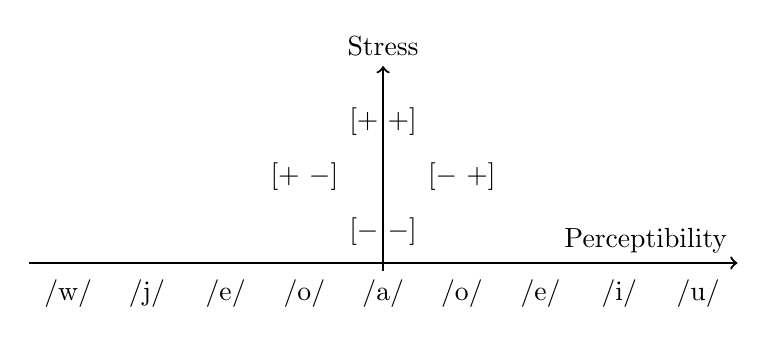
\begin{tikzpicture}
		\def\h{0.68}
		
		\def\tick#1#2#3{\draw[thick,#2] (#1+.09) --++ (0,-.18) node[below=-2pt] {\strut #3};}
		

		%\fill[left color=myred, right color=myyellow] (5,0) rectangle (35,\h);
		%\fill[left color=myyellow,right color=mygreen] (35,0) rectangle (50,\h);
		%\fill[left color=mygreen,right color=myyellow] (50,0) rectangle (65,\h);
		%\fill[left color=myyellow,right color=myred] (65,0) rectangle (95,\h);

		\draw[->,thick] (0,-.1) -- (0,2.5) node[above] {Stress};

		\node[above ] at (0,.1) {[$- \ -$]};
		\node[above] at (-1,.8) {[$+\ -$]};
		\node[above] at (1,.8) {[$-\ +$]};
		\node[above] at (0,1.5) {[$+\ +$]};
	
		
		% INTENSITY
		\draw[->,thick] (-4.5,0) -- (4.5,0) node[above left] {Perceptibility};
		%\draw[->,thick] (20,0) -- (15,0) node[below right=-3,scale=1.1] {};

		%\node[below=-4,scale=0.9] at (15,-3.5) {\strut {$+$}};
		%\node[below=-4,scale=0.9] at (46,-.1) {\strut {$-$}};
		%\node[below=-4,scale=0.9] at (46,1.4) {\strut {$+$}};
		%\node[below=-4,scale=0.9] at (84,-3.5) {\strut {$+$}};
		\node[below=-4] at ( -4,-0.2) {\strut {/w/}};
		\node[below=-4] at ( -3,-0.2) {\strut {/j/}};
		\node[below=-4] at ( -2,-0.2) {\strut /\textsubarch{e}/};
		\node[below=-4] at ( -1,-0.2) {\strut /\textsubarch{o}/};
		\node[below=-4] at ( 0,-0.2) {\strut {/a/}};
		\node[below=-4] at ( 1,-0.2) {\strut /\textsubarch{o}/};
		\node[below=-4] at ( 2,-0.2) {\strut /\textsubarch{e}/};
		\node[below=-4] at ( 3,-0.2) {\strut /\textsubarch{i}/};
		\node[below=-4] at ( 4,-0.2) {\strut /\textsubarch{u}/};

	\end{tikzpicture}

\caption{Perceptibilidad.}
\label{fig:percep}
\end{figure}

Para ayudarnos en la evaluación de uniones vocálicas, definimos una nueva variable. Esta la usaremos para establecer la posición de las vocales. Para ello, asignamos coordenadas a cada fonema según su punto de articulación en la cavidad bucal (\Cref{fig:trapez}). Con esta configuración, la posición más central con apertura media sería el origen, el eje de abscisas representaría la frontalidad y la apertura se distribuiría a lo largo del eje de ordenadas. Estas coordenadas servirán más adelante para ordenar los desplazamientos entre fonemas. Hemos encontrado que un sistema de coordenadas ortonormal con valores aproximados de las posiciones produce buenos resultados. A la luz de los experimentos llevados a cabo para optimizar los resultados, las coordenadas $\textipa{/i/} = (-1, 1)$, $\textipa{/e/} = (-1, 0)$, $\textipa{/a/} = (0, -1)$, $\textipa{/u/} = (1, 1)$ y $\textipa{/o/} = (1, 0)$ son suficientes para conseguir la escansión óptima del corpus de sonetos con el que  hicimos las pruebas.

Nótese que los valores provistos no representan de manera exacta la relación con la articulación física de los sonidos. En otras palabras, no estamos asignando un valor numérico realmente, sino ordenando los pares vocálicos según la distancia entre sus componentes. Asimismo, la marcas solo resulta relevante a igualdad de condiciones entre varias uniones, como voto de calidad para decidirse por una u otra.

\begin{figure}[!ht]
	\centering
		\begin{tikzpicture}[line cap=rect] 
		\def\h{0.68}
		
		\def\tick#1#2#3{\draw[thick,#2] (#1+.09) --++ (0,-.18) node[below=-2pt,scale=1] {\strut #3};}
		
		%draw[-,thick,myred] (-.5,1.5) -- (5.5,1.5) node[below right=-3,scale=1.1] {};
		%\draw[-,thick,myred] (2.5,3.5) -- (2.5,-.5) node[below right=-3,scale=1.1] {};
		%\draw[step=12.5cm,gray,very thin] (-5,-5) grid (55,35);
		%\fill[left color=myred, right color=myyellow] (5,0) rectangle (35,\h);
		%\fill[left color=myyellow,right color=mygreen] (35,0) rectangle (50,\h);
		%\fill[left color=mygreen,right color=myyellow] (50,0) rectangle (65,\h);
		%\fill[left color=myyellow,right color=myred] (65,0) rectangle (95,\h);
		\draw[thick,->,myred] (-3.2,0) -- (3.2,0) node[anchor=north west] {Localización};
		\draw[thick,->, myred] (0,-2.5) -- (0,2.5) node[anchor=south east] {Apertura};
		\foreach \x in {-2, -1, 1, 2}
		\draw (\x cm, 1pt) -- (\x cm,-1pt) node[anchor=north] {};
	
		
		\draw[-,thick,black!10] (0,2) -- (2.7,2) -- (2.7, -2) -- (0, -2) -- (-2.7, 2) -- (0, 2) node[below right=-3,scale=1.1] {};		
		\draw[-,thick,black!10] (-2.02,1) -- (2.7,1) node[below right=-3,scale=1.1] {};
		\draw[-,thick,black!10] (-0.67,-1) -- (2.7,-1) node[below right=-3,scale=1.1] {};		

		\draw[-,thick,black!10] (0,2) -- (2.7/2,-2) node[below right=-3,scale=1.1] {};

			\foreach \y in {-2, -1, 1, 2}
		\draw (1pt,\y cm) -- (-1pt,\y cm) node[anchor=east] {};
		%\draw (0pt, 0pt) node[anchor=north east] {0};
	
		\node[scale=1] at (-2.55,1.9) {\strut {i}};
		\node[scale=1] at (2.4,1.8) {\strut {u}};
		\node[scale=1] at (-1.45,.25) {\strut {e}};
		\node[scale=1] at (2.6,.12) {\strut {o}};
		\node[scale=1] at (1.8,-1.87) {\strut {a}};
		
		
	\end{tikzpicture}
	\caption{Vocales en el trapecio bucal.}
	\label{fig:trapez}
\end{figure}

Además de estas variables requeridas por los algoritmos, definiremos otras por conveniencia, con las que nombrar colectivamente a vocales\index{vocal}, vocoides\index{vocoide} y vocales cerradas\index{vocal!cerrada}. De este modo, nos referiremos después a ellas sin necesidad de volver a nombrarlas de nuevo de manera explícita.

A continuación definimos las clases auxiliares (\cref{list:clasesauxiliares}). La primera de ellas, a la que llamaremos clase \Valores, define objetos cuyos atributos son rasgos de la palabra. Estos son la propia palabra, su categoría gramatical, una lista de sus sílabas transcritas fonológicamente, rasgos sintáctico-gramaticales adicionales —persona y caso, por ejemplo— y si es tónica. La segunda, \Verso, contiene la información que permite caracterizar el verso: sus sílabas, el tipo de ambigüedad, el recuento silábico y la rima, tanto asonante como consonante. Las sílabas están marcadas para distinguir entre vocales silábicas y no silábicas, de manera que representa implícitamente los núcleos vocálicos del verso y los acentos prosódicos, esto es, la caracterización propia del ritmo.

\begin{algorithm}[!ht]
	\caption{Clases auxiliares.}\label{list:clasesauxiliares}
	\Fclase{\Valores{}}{
		\text \is \cadena \;
		\pos \is \cadena \;
		\phon \is \lista \;
		\feats \is \diccionario \;
		\dep \is \lista \;
		\ton \is \booleano
	}
	\;
	\Fclase{\Verso{}}{
		\slbs \is \lista \;
		\amb \is \entero \;
		\recuento \is \entero \;
		\asson \is \cadena \;
		\conss \is \cadena
	}
\end{algorithm}

\section{Prosodia gramatical}
Con esto, abordaremos la primera clase funcional, que servirá para definir la prosodia del verso sin considerar las licencias poéticas. La definición es simple. La clase \Frase recibe una línea de texto que preprocesa\footnote{En la implementación en Python, el resultado de preprocesar la línea se somete a un paso adicional antes de ser utilizado, ya que detectamos errores puntuales en el módulo de análisis morfosintáctico que conviene enmendar. Sirva esto también como elogio a la labor de los miembros del proyecto Stanza NLP, quienes resolvieron con premura todos los fallos que reportamos.} para obtener el verso final ya listo para trabajar con él. En este, identificamos los rasgos de las palabras y, apoyándonos en ellos, buscamos los acentos prosódicos. El resultado lo dejamos en una variable que contiene una lista de palabras, cada una de las cuales es, a su vez, una lista de sílabas. Estas están representadas por su transcripción fonética. En cuanto a la prosodia, la sílaba acentuada no se marca en todas las palabras sino solo en las tónicas.

\begin{algorithm}[!ht] %or another one check
	\caption{Clase \texttt{Frase}.}\label{list:playline}
	\Fclase{\Frase{}}{
			\Fmetodo{\inicializa{línea}}{
			\fixedverse   \gets \preprocess{línea}\;
			\words \gets \FindPS{versolisto}
		}
	}
\end{algorithm}

Veamos en qué consisten los métodos de la clase. En el preprocesado, alteramos las palabras de manera que resulte más conveniente su análisis. Por ejemplo, las palabras homógrafas de clases tónicas y átonas pueden ser analizadas por el programa incorrectamente, lo que provoca errores en el análisis del ritmo. Entre dos palabras átonas o entre dos tónicas, el problema es irrelevante, en tanto que no afecta a la prosodia desde nuestro punto de vista\footnote{Esto es una idealización en la que solo tenemos sílabas tónicas y átonas. En realidad, existe una gradación de la intensidad de la acentuación, por lo que existen diferencias entre dos palabras acentuadas o dos átonas. En esta diferenciación sí influye la categoría gramatical de la palabra y su función sintáctica.}. Así, empezaremos haciendo algunas correcciones \textit{ad hoc}. Por ejemplo, el imperativo singular de \textit{parar} plantea una situación problemática en tanto que el programa de análisis morfosintáctico tiende a confundirlo con la preposición\index{preposición}. No obstante, tenemos al menos un caso del que se infiere la categoría gramatical gracias a la puntuación. En español, la preposición es el núcleo sintáctico de un sintagma preposicional que no suele romperse con la puntuación salvo para introducir apartes (\ref{exe:para}). Dadas las limitaciones estructurales que impone el verso, su empleo resulta más inusual que en el texto narrativo, Además, si el aparte no es retórico, este se señala mediante una acotación\index{acotación}. Por lo tanto,  si encontramos un \textit{para} seguido de coma y un sintagma nominal, asumiremos que, probablemente, se trate del imperativo de \textit{parar} con la coma propia del vocativo.

\begin{exe}
	\ex\label{exe:para}Para, digamos, eso.
\end{exe} 

Si se trata de esto, es posible engañar al programa haciéndole creer que la palabra es un nombre propio, por lo que será marcada como tónica. No supondría un problema que, como es común, el vocativo fuera otro nombre propio, ya que, al ir separados por coma el nombre verdadero y el impostado, no sería entendido como un nombre compuesto y, por lo tanto, el primero no perdería su calidad tónica.

\begin{algorithm}[!ht] %or another one check
	\caption{Preprocesado.}\label{list:preprocess}
	\Fmetodo{\preprocess{línea}}{
		\linea{$\langle\text{para,}\rangle$} \gets $\langle\text{Ppara,}\rangle, \forall \langle\text{para}\rangle \in l\acute{\imath}nea$\;
		\symbols \gets \{\textlangle{}(\textrangle: \textlangle{}. \textrangle, \textlangle{})\textrangle: \textlangle{}. \textrangle, \textlangle{}—\textrangle: \textlangle{}. \textrangle , \textlangle{}…\textrangle: \textlangle{}. \textrangle, \textlangle{}«\textrangle: \textlangle \textrangle, \textlangle{}»\textrangle: \textlangle \textrangle, ...\\ \Indp
		 \textlangle{}õ\textrangle: \textlangle{}o\textrangle, \textlangle{}æ\textrangle: \textlangle{}e\textrangle, \textlangle{}à\textrangle: \textlangle{}a\textrangle, \textlangle{}ì\textrangle: \textlangle{}e\textrangle, \textlangle{}ì\textrangle: \textlangle{}i\textrangle, \textlangle{}ò\textrangle: \textlangle{}o\textrangle, \textlangle{}ù\textrangle, ...\}\;   \Indm
		 \uIf{línea \is $\emptyset$}{\verso \gets $\langle\emptyset\rangle$}
		  \uElse{
		  	\linea \gets \CorrigeP{línea} \;
		  	\linea \gets \PLN{línea} \;
		  	\verso \gets $(palabra_0, ..., palabra_n ), \forall palabra_i \in \text{linea}$
		  }
	  \Return{\SetFeats{verso}}
	}
\end{algorithm}

A continuación, corregimos la ortotipografía para no tener que considerar situaciones excepcionales. Esto incluye asegurarse de que el espaciado sea  apropiado —por ejemplo, que no haya dos espacios seguidos o entre una palabra y la puntuación de cierre o, por el contrario, ponerla si falta entre la puntuación de cierre y el inicio del siguiente grupo de palabras. Asimismo, 
simplificamos los signos ortográficos, tanto la puntuación como los diacríticos\index{diacrítico}, para reducir el número de casos a considerar durante el procesado\footnote{En el algoritmo propuesto, hemos circunscrito el diccionario de sustituciones a una muestra porque la intención es ilustrar la idea y no detallar todos los casos. No obstante, se encuentra una forma más completa en la implementación para el computador en \Cref{list:libscansion}.}. También transliteramos aquí marcas diacríticas ajenas a la ortografía española.

Solo resta aplicar el procedimiento de análisis morfosintáctico y almacenar los resultados en una lista ordenada según la posición de las palabras en el verso. Dado que recurrimos a una biblioteca de análisis morfosintáctico externa, necesitamos adaptar el formato a nuestras necesidades, por lo que introducimos un módulo \texttt{FijaRasgos} para dejar la salida de la subrutina en una forma más manejable. De nuevo, este módulo se trata de una abstracción que debe concretarse de manera diferente para cada caso específico\footnote{Por ejemplo, en \Cref{list:libscansion} para la biblioteca \texttt{Stanza}.}. Se trata de, a partir de la lista de palabras obtenida, componer otra en la que cada uno de sus elementos sea un objeto de la clase \Valores con los rasgos necesarios.

Una vez dispuesta cada palabra del verso para que exhiba la información relevante, establecemos la prosodia del verso con arreglo a los acentos internos y la morfosintaxis de las palabras que lo componen. Este paso es crítico y, de su correcta solución junto con la evaluación de las sinalefas, depende determinar el ritmo métrico satisfactoriamente en la mayoría de los versos. Asimismo, es un paso que entraña ciertas dificultades de carácter técnico —al contrario que la resolución de uniones vocálicas, que es conceptual, como veremos—. La razón de las posibles complicaciones es la necesidad de categorizar las palabras del verso y considerar sus relaciones sintácticas. Si bien existen herramientas que automatizan la tarea, estas no son del todo precisas. Por lo tanto, aquí habremos de introducir una serie de soluciones al efecto para sortear fallos en el análisis gramatical. Lamentablemente, esto obliga a complicar este paso para contemplar una miríada de casos excepcionales que, de otra manera, habrían podido resolverse de una forma más elegante.

 \begin{algorithm}[!ht]
 	\caption{Búsqueda de acentos prosódicos del verso (I).}\label{list:findps1}
 	\Fmetodo{\FindPS{palabras}}{
 		\tonicas \gets $\{a_i\}^{n}_{i=1},\:a_i\:\in \text{categorías tónicas}$\;
 		\atonas \gets $\{b_i\}^{n}_{i=1},\:b_i\:\in \text{palabras átonas}$\;
 		\tons \gets $\{c_i\}^{n}_{i=1},\:c_i\:\in \text{palabras tónicas}$\;
 		\ant \gets $\emptyset$ \; 
 		\unidades \gets \False \;
 		/* \Cref{list:findps2} */
 	}
 \end{algorithm}

Aquí debemos crear listas de categorías gramaticales y palabras átonas y tónicas de acuerdo con lo expuesto en el capítulo que dedicamos a los aspectos teóricos de la métrica. Asimismo, definimos una variable booleana $unidades$, que emplearemos, en caso de encontrar numerales, para identificar los órdenes de magnitud superior a la unidad en palabras compuestas.

A continuación,  procedemos a recorrer las palabras del verso en sentido inverso; esto es, desde la última a la primera. La razón para hacerlo así y no en su orden natural de lectura es que, en caso de compuestos de elementos de idéntica categoría, como numerales o nombres propios,  el acento recae en la última palabra y son átonas las precedentes (\Cref{list:findps2}). Por lo tanto, partimos de que la primera palabra que encontremos de las categorías susceptibles de agrupación es tónica con independencia de que forme parte de una estructura más compleja de palabras de su clase. De seguir la disposición natural del verso, al dar con una palabra semejante no podríamos determinar de antemano si lleva o no acento, ya que se haría necesario cotejarla con las palabras subsiguientes para dilucidar si forma parte de una composición.

Partimos de la premisa de que la palabra es átona; esta suposición variará en función de las pruebas a las que la someteremos. En \Cref{list:findps2}, definimos por conveniencia algunas variables descriptivas de los valores que les asignamos. Estas no son necesarias desde una perspectiva funcional, pero mejoran la legibilidad. Se comprueba primero si la palabra es la última del verso —la primera en nuestra lista de palabras invertida—, contiene vocales con tilde o es alguna de las que hemos definido como  tónicas de manera inequívoca. En ambos casos, habremos de concluir que la palabra es tónica. De no cumplirse ninguno de las dos, constatamos que la palabra pertenezca al conjunto de átonas que definimos y, de ser cierto, no necesitamos hacer nada más salvo asignar un valor vacío a la palabra anterior para la próxima iteración, pues ya habíamos marcado la palabra como átona por defecto. Si tampoco es el caso, necesitaremos explorar los rasgos gramaticales de las palabras y su contexto sintáctico para encontrar sus características prosódicas. Dado que es necesario considerar un número significativo de posibilidades, lo detallaremos en un algoritmo aparte.

\begin{algorithm}[!ht]
	\caption{Búsqueda de acentos prosódicos del verso (II).}\label{list:findps2}
	\words \gets $\{b_1\}^n_{i=1}, b_1=a_{(n+1)-i}, a_i \in \text{palabras}$ \;
	\For{$palabra_i \in palabras$}{
		\ton \gets \False \;
		\texto \gets $palabra_{texto}$ \;
		\pos \gets $\text{palabra}_{\text{categorí}}$ \;
		\feats \gets $\text{palabra}_{\text{rasgos}}$ \;
		\uIf{$i = 0 \wedge  \exists x \in \text{texto}, x \in \{\acute{a}, \acute{e}, \acute{\imath}, \acute{o}, \acute{u}\} \wedge \text{texto} \in t\acute{o}nicos$}{$\ton \gets \True$}
		\uElseIf{$texto \in \text{átonas}$}{$\text{palabra}_0 \gets \langle{}\rangle$}
		\uElse{/* \Cref{list:findps3} */}
		$\word_{\text{tónica}}$ \gets \text{tónica} \;
		\pos$_0$ \gets \text{categoría}      
	}
\end{algorithm}

Empezamos por marcar por defecto como acentuadas las palabras pertenecientes a categorías que, en principio, consideramos tónicas (\Cref{list:findps3}). No obstante, modificaremos después esta clasificación preliminar si el contexto de la palabra lo requiere. Para ello, iniciamos una serie de comprobaciones, empezando por determinar si la palabra es un numeral. Sabemos que en números compuestos solo es tónica la última parte. Esto es, pongamos que tenemos, por ejemplo el número 333, la transcripción será \ipa{/tRes.Tjen.tos tRe\textsubarch{i}n.ta\textsubarch{i} ˈtRes/}. Debido a eso, empezamos por asegurarnos de que la palabra anterior —recordemos que hemos invertido el orden, por lo que la palabra precedente en nuestro orden de verificación es la que sigue en la oración— no sea numeral. Si no lo es, la marcamos como tónica y, si es del orden de magnitud de las unidades, lo indicamos. La razón para esto es evitar que dos numerales independientes se evalúen como una agrupación. Esto es, por ejemplo, \textit{uno, dos y tres}, al contrario que un número compuesto, tendría todas sus palabras acentuadas. En teoría, esto no está circunscrito a las unidades, ya que lo mismo sucedería con, por ejemplo \textit{veinte y treinta}. Sin embargo, si los primeros casos son escasos, los segundos lo son más. Para refinar la clasificación podríamos proponer comprobar si estamos ante órdenes de magnitud equivalentes (\textit{uno y dos}). Sin embargo, casos como \textit{cuarenta y dos} necesitarían contextualización semántica. Esto es, estaríamos ante un único grupo con acento en \textit{dos} si, por ejemplo, una persona está dando su edad, pero serían dos grupos acentuados si el interpelado se refiere a la suya (40) y la de su hijo (2). Asimismo necesitamos recurrir a la ortografía para diferenciar \textit{trescientos treinta y tres} de \textit{trescientos, treinta y tres}, la primera con un solo acento en \textit{tres} y la segunda con los tres componentes acentuados al comenzar. Esto es empero discutible, ya que se cumple si aludimos a \textit{333}, pero no si representa \textit{300, 33}, en cuyo caso \textit{treinta} sería átona, o  \textit{330 y 3}, en la que \textit{trescientos} sería átona, pero \textit{treinta} y \textit{tres} tónicas

No todos los componentes de la unidad han de ser numerales por sí mismos. Por eso la siguiente comprobación es si la palabra es la conjunción \textit{y} antes de numeral, lo que la convertiría en parte del grupo, no embargante lo dicho en el párrafo anterior. Si es así, forzamos su clasificación a numeral de manera que en la próxima iteración tenga en cuenta este contexto. Si tampoco es el caso, cotejamos la palabra con el conjunto de voces necesariamente átonas y, de estar en él, la marcamos como tal. 
 
\begin{algorithm}[!ht]
	\caption{Búsqueda de acentos prosódicos del verso (III).}\label{list:findps3}
		\If{categoría $\in$ categorías\_tónicas}{
			$\ton \gets \True$
		}
		\uIf{categoría =  `numeral'}{
			\uIf{anterior $\neq$ `numeral'}{
				\ton \gets \True \;
				\uIf{texto $\in$ unidades}{\unidad \gets \True}
				\uElse{\unidad \gets \False}
			}
			\uElseIf{texto $\in$ unidades}{
				\If{unidad $\is$ \True}{\ton \gets \True}
				\unidad \gets \True}
			\uElse{\unidad \gets \False}
		}
		\uElseIf{$\text{texto} = \langle{}y\rangle \wedge \text{anterior } \is \text{ numeral}$}{
			\pos \gets `numeral' \;
			\ton \gets \False
		}
		\uElseIf{$\text{texto} \in \acute{a}tonas$}{$\text{palabra}_0 \gets \langle{}\rangle$}
		/* \Cref{list:findps4} */   
\end{algorithm}

Si no se ha cumplido ninguna de las condiciones anteriores, la prueba consistirá en verificar si se trata de un \textit{determinante}\index{determinante}\footnote{En la implementación en Python, se confunde hasta cierto punto esta categoría con los pronombres. El programa encargado del etiquetado morfosintáctico cometía algunos errores, por lo que fue necesario introducir cambios para tenerlos en cuenta. No se entienda esto como una toma de postura a favor de la hipótesis del sintagma determinante \parencite{bernstein2001} frente al nominal —una controversia sobre la que no tenemos elementos de juicio y dejamos a los expertos que sí los tienen—, sino como una mera cuestión práctica. En esta aproximación idealizada, por el contrario, damos por supuesto que el lector no cometerá esos fallos y nos atendremos a la gramática.} y lo marcaremos como átono si no es indefinido o demostrativo\index{demostrativo}. Si tampoco se da esta situación, comprobamos a continuación si se trata de un pronombre. De ser así, se hace necesaria una distinción más detallada. Primero miramos si es un pronombre objeto o reflexivo, en cuyo caso será átono. En el caso de que tuviéramos un verbo con pronombres clíticos, el etiquetador gramatical analizaría sus elementos por separado. Si se trata de un objeto indirecto o directo que no es parte de un sintagma preposicional, asumimos que es un pronombre   

Podría ser que tuviéramos un verbo\index{verbo} con clítico\index{clítico} clasificado como tal y, para ello, verificamos si la palabra acaba en un pronombre átono, pero sin ser toda ella uno, de manera que, si se cumple, tendremos un compuesto cuya primera parte es tónica. Otra posibilidad es que estemos ante un posesivo. En ese caso, debemos distinguir la clase, pues los artículos son átonos mientras que los pronombres son tónicos aun siendo homógrafos. Introduciremos también una condición que obligue a ignorar las operaciones subsiguientes en caso de tener un indefinido o un demostrativo, ya que estos son tónicos. Si la palabra no satisface las condiciones anteriores, miramos si actúa como objeto directo o indirecto y, de ser así, si es un pronombre átono. A continuación, buscamos amalgamados \textit{con + migo/tigo/sigo} y, tras esto los relativos. En cualquier otro caso, la palabra permanece marcada como tónica.
\begin{algorithm}[!ht]
	\caption{Búsqueda de acentos prosódicos del verso (IV).}\label{list:findps4}
	\uElseIf{categoría \is determinante}{
		\If{$\text{rasgos}_{\text{tipo}} \is \neg\text{demostrativo} \vee  \text{rasgos}_{\text{tipo}} \is \neg\text{indefinido}$}{\ton \gets \False}}
	\uElseIf{categoría \is pronombre}{
		\uIf{$\text{rasgos}_{\text{caso}}$ \is \text{objeto}}{
			\uIf{$\text{texto} \notin \text{pronombres átonos}$}{\ton \gets \True}
			\uElse{\ton \gets \False}
		}
	\uElseIf{`-igo' $\in$ texto}{\ton \gets \True}
	\uElseIf{texto = \textlangle{}donde\textrangle $\vee rasgos_{tipo} \in \{Int, Rel\}$}{\ton \gets \False}}
 	/* \Cref{list:findps5} */   
\end{algorithm}

La siguiente comprobación incluye sustantivos\index{sustantivo} o fórmulas de tratamiento\index{fórmula de tratamiento}, cualesquiera que sean sus categorías gramaticales; esto es, incluimos aquí formas sustantivas como \textit{don} o \textit{doña} pero también sustantivos como \textit{santo} o su variante apocopada \textit{san}. La razón es que, en combinación con nombre propio, reproducen el comportamiento prosódico de otros nombres propios antepuestos: son átonos. Al igual que los numerales, solo el último nombre propio de una forma compuesta lleva acento. Como estamos leyendo el verso desde el final hacia el principio, crearemos una variable que indique si la palabra examinada anteriormente es un nombre propio, de manera que si este es el caso, la que estemos analizando tras ella será átona. En cualquier otro caso, no necesitaremos  cambiar nada, ya que el sustantivo será palabra tónica.

Si no se ha cumplido tampoco la condición previa, la siguiente a comprobar es si la palabra es un adverbio\index{adverbio}. En caso de que efectivamente lo sea, la marcaremos como átona si funciona como conjunción o es parte de una compleja \parencite[24]{quilis2013}.

\begin{algorithm}[!ht]
	\caption{Búsqueda de acentos prosódicos del verso (V).}\label{list:findps5}
	\uElseIf{$\text{categoría} \is \text{sustantivo} \vee \text{texto} \in \text{tratamientos}$}{
		\uIf{$\text{texto} \in \text{tratamientos} \wedge \text{anterior}  \is \text{nombre propio}$}{
			\ton \gets \False \;
			\ant \gets $\emptyset$
		}
	}
	\uElseIf{\text{categoría} \is \text{adverbio}}{
		\uIf{$\text{texto} \is \text{adverbio} vee \text{texto} \in \text{adverbio}$}{\ton \gets \False}
	}
	\ant \gets \text{categoría} \;
	/* \Cref{list:findps11} */   
\end{algorithm}

Una vez hechas todas las comprobaciones, procedemos a marcar la conjunción \textit{y}, de manera que podamos reconocerla en la transcripción fonológica aun sin disponer de información gramatical.

Tenemos una buena estimación del ritmo del verso, pero esta presenta algunas deficiencias. Por una parte, hemos analizado las palabras de manera individual y, por otra, no hemos tenido en cuenta las demandas del metro. En la lengua oral, las palabras no son independientes unas de otras, sino que producen un sonido continuo que difumina sus márgenes. Aquí volvemos a las nociones de fonética acústica que vimos en la parte teórica.

\begin{algorithm}[!ht]
	\caption{Tratamiento de la conjunción \emph{y}.}\label{list:findps11}
	\words \gets $\{b_1\}^n_{i=1}, b_1=a_{(n+1)-i}, a_i \in \text{palabras} $ \;
	\For{$\text{palabra}_i \in \text{palabras}$}{
		\If{$i < n-1 \vee \text{palabra}_{\text{texto}} = \langle y\rangle$}{
			\uIf{$x \in \text{vocales} \forall x \in \{\text{palabras}_{i-1, fon._{n,m}}, \text{palabras}_{i+1, fon._{0,0}}\}$}{\words$_{i,fon._0}$ \gets $\langle y\rangle$}
		}
	}
	\Return{$\{\text{palabra}_i\}^n_{i=1}, \forall \text{palabra} \in \text{palabras}$}
\end{algorithm}

Si tomamos el fonograma de un enunciado, observamos fenómenos coarticulatorios\index{coarticulación} entre palabras. Así, las sílabas fonéticas de, por ejemplo, \textit{álbum abierto}, no se corresponden con las gramaticales (\textit{al·bum·a·bier·to}) sino que se pronunciará como (\textit{al·bu·ma·bier·to}). Si bien la unión entre vocal y consonante no tiene consecuencias en la escansión del verso, el contacto intervocálico altera a menudo la pronunciación. La sinalefa, cuyas características mencionamos en el capítulo dedicado a la fonología, y su efecto en el verso, en el dedicado al metro, reduce de forma natural la medida del verso. Por otra parte, si el metro lo requiere, el poeta ajustará el número de sílabas forzando diptongos\index{diptongo} mediante sinéresis\index{sinéresis} o hiatos\index{hiato} mediante diéresis\index{diéresis}. Así pues, debemos considerar estos fenómenos tomando las sílabas del verso como un flujo continuo y no como una serie de palabras aisladas e independientes.

\section{Ajustes métricos}
Para hacer esto, definimos una nueva clase \MetroVerso hija de \Frase que, por lo tanto, hereda los métodos y atributos de esta. Recordemos: $versolisto$ y $palabras$, dos listas en el que la primera contiene información gramatical de cada palabra del verso y la segunda listas correspondientes a las sílabas de cada una de las palabras con los acentos prosódicos ya marcados. Asimismo, definimos una lista ordenada con metros, que se usará en caso de que no se proporcione de manera explícita el parámetro $esperadas$ para establecer el orden de preferencia de los metros para los que se intentará escandir el verso. Esto es, intentaremos ajustar el verso para que tenga tantas sílabas como indica el primer elemento de la lista; si no es posible, como el segundo; después el tercero, etc.

Antes de definir los atributos de la clase, creamos una condición para asegurarnos de que el verso contiene al menos una palabra. Esto permite atajar ya aquí esta contingencia para evitar arrastrarla en el proceso, lo que complicaría su localización y obligaría a hacer excepciones más adelante.

Los atributos de la clase son las sinalefas\index{sinalefa}, representadas en una lista de estas, así como la prioridad de cada una, obtenida de aplicar un método al efecto. Asimismo obtenemos una estimación de la longitud del verso en condiciones normales, esto es, haciendo las sinalefas obligatorias o, en nuestro caso, aquellas con una prioridad que supere un umbral determinado, como veremos más adelante. Otro método obtiene las características prosódicas del verso, a saber: las sílabas que lo componen, su rima y valores derivados como el número de sílabas y la rima parcial. Por último extraemos los núcleos silábicos del verso y traducimos estos a una notación binaria en función de si llevan o no acento para representar el patrón rítmico.

\begin{algorithm}[!ht]
	\caption{Ajustes métricos.}\label{list:VerSeMetre1}
	\Fclase{\MetroVerso{\Frase}}{
		\comunes \gets(6, 7, 8, 11, 9, 10, 12, 13, 5, 4, 3) \;
		\Fmetodo{\inicializa{línea, esperadas \gets comunes}}{
			\If{$\exists palabra$ $\in$ palabras}{
				\sinalefas \gets \EncuentraSinalefas{palabras} \;
				\estimacion, \esperadas \gets \AjustaEsperadas{palabras, sinalefas, esperadas}\;
				\verso \gets \AjustaMetro{palabras, esperadas}\;
				\silabas \gets \text{verso.sílabas} \;
				\ambiguedad \gets \text{verso.ambi} \;
				\asonancia \gets  \text{verso.asonancia} \;
				\rima \gets \text{verso.consonancia} \;
				\cuenta \gets \text{cuenta.recuento} \;
				\nucleos \gets \EncuentraNucleos{sílabas} \;
				\ritmo \gets \EncuentraRitmo{núcleos}
			}
			\Else{
				\sinalefas, \esperadas, \silabas  \gets [] \;
				\estimacion, \cuenta \gets 0 \;
				\ambiguedad, \asonancia, \rima \gets \False \;
				\nucleos, \ritmo \gets $\emptyset$
			}
		}
	}
\end{algorithm}

Desglosemos antes de nada las funciones que hemos utilizado aquí, para, una vez tengamos las partes principales, hacer lo propio con las subrutinas que las componen y explorarlas analíticamente. Hacemos una estimación del número de sílabas del verso. Para ello necesitamos antes la cuenta de contactos vocálicos entre palabras para conocer las sinalefas potenciales. Si bien es posible que se dé una dialefa\index{dialefa} entre límites vocálicos de palabra adyacentes, hay casos en los que, como vimos en la parte teórica, esto contravendría la pronunciación natural del verso. Tales pares de sílabas deben de ser considerados \textit{a priori} como una sola sílaba métrica y, solo de manera excepcional, se escandiría el verso atendiendo a su división silábica gramatical. Por lo tanto, definimos un método dedicado a analizar el verso en busca de sinalefas posibles (\Cref{list:VerSeMetre2}).

\begin{algorithm}[!ht]
	\caption{Búsqueda de vocales en contacto (I).}\label{list:VerSeMetre2}
	\Fmetodo{\EncuentraSinalefas{palabra, h \gets \False}}{
		\sinalefas \gets ()\;                                                     
		\preferencia, \desplazamiento \gets  0 \;
		\For{$\text{palabra}_i \in \text{palabras}$}{
			\sV, \sC, \s \gets $\text{palabra}_0$, $\text{palabras}_{i-1, n}$, \False \;
			\If{$i \neq 0 \wedge \forall x \in \{C_n, V_0\}, x \in \text{vocálicas}$}{
				\If{$i = 1 \wedge \text{palabras}_0 \in \{i, o\} \wedge V_0 \in \text{vocales}^{+\textsc{tón}}$}{
					\preferencia \gets $\text{preferencia} - 8$}
				\position \gets $(idx -1, \lvert \text{palabras}_{idx-1} - 1)$ \;
				\If{$\text{palabra} \in \{(i), (e)\} \wedge \lvert \text{palabras}\rvert > idx + 2$}{
					\If{$C_n \in \text{vocálicas}$}{
						\If{$\text{palabras}_{idx+1, 0, 0} \in \text{vocálicas}$}{\s \gets \True}
					}
				}
				\ElseIf{$\text{fonema} \in \text{vocálicas}, \forall \text{fonema} \in \{C_n, V_0\}$}{
					\perc \gets  $\text{perceptibilidad}_{C_n}$\;
					\If{$\lvert C\rvert > 1 \wedge C_{-2} \in \text{perceptibilidad}$}{$previous\_val$ \gets $\text{perceptibilidad}_{C_{-2}}$}
					\Else{\anterior \gets $\text{perceptibilidad}_{C_{n}}$}
					\If{$\lvert V\lvert > 1 \wedge V_1 \in \text{perceptibilidad}$}{\siguiente \gets $\text{perceptibilidad}_{V_1}$}
					\Else{\siguiente \gets $\text{perceptibilidad}_{V_0}$}
					\If{$\text{anterior} \leq  \text{perc} \wedge \text{perc} \leq \text{perceptibilidad}_{V_0} \vee \text{anterior} \geq \text{perc} \wedge \text{perc} \geq \text{perceptibilidad}_{V_0} \wedge \text{siguiente} \leq \text{perceptibilidad}_{V_0} \vee \text{anterior} \leq \text{perc} \wedge \text{perc} > \text{perceptibilidad}_{V_0} \wedge \text{perceptibilidad}_{V_0} \geq \text{siguiente}$}{\s \gets \True}
				}
			}
			\If{s}{
				\If{$\forall x^{-\textsc{tón}} \in \{C, V_0\} \wedge C_n = V_0$}{
					\If{$\exists x \in \{['o'], ['y'], ['u'], ['e']\} \wedge x \in \{\text{palabra}, \text{palabras}_{i-1}\} $}{\preferencia \gets  $preferencia -1 $}
					\ElseIf{$\lvert V\rvert > 1 \wedge V_1 \in \{\text{vocoides}\} $}{
						\preferencia \gets  $\text{preferencia} - 2 $}
				}
				\sinalefas \gets \text{sinalefas} + (\text{posición}, \PreferenciaSinalefa{C, V, \text{preferencia}}, C, V)
			}
			\desplazamiento \gets $\text{desplazamiento} + \lvert\text{palabra}\rvert $  \;     
		}
		/* \Cref{list:VerseMetre3} */                                                    
	}		   
\end{algorithm}

Aquí se trata de componer una lista de posiciones donde es factible la sinalefa\index{sinalefa}. Asimismo, hay que definir otra lista para contener la palabra precedente a la que estamos evaluando. Antes de hacerlo, inicializamos a cero la preferencia de la sinalefa y la cuenta del desplazamiento dentro del verso.  Con esto, empezamos a recorrer las palabras, que, recordemos, representábamos a su vez como listas de sílabas. Para simplificar, pensemos en la sinalefa como dos segmentos, uno inicial, compuesto de una posición no silábica más una nuclear, y uno final, compuesto de una posición nuclear junto a una no silábica, como la restricción de que una y solo una de las posiciones nucleares estará ocupada y ninguna de las partes estará completamente vacía. La posición nuclear solo acepta vocales puras, mientras que las no silábicas solo aceptan vocoides\index{vocoide}. Los posibles segmentos son $C N - V$, $C - N V$, $N - V$, $C - N$, donde $V$ representa el segmento vocálico y $C$ el semiconsonántico o semiocálico, sin preocuparnos  ahora de cuál de ellos contiene el núcleo. La primera condición que establecemos es que, obviamente, la sinalefa no puede darse en la sílaba inicial del verso, pues no hay palabra precedente con la que pueda formarla. En cualquier otro caso, la palabra actual debe comenzar por sonido vocálico, como también vocálico debe ser el final de la anterior. Si esto es cierto, confirmamos que se trata de una sinalefa potencial para asignarle un rango de preferencia.

Primero  marcamos la posición donde comienza la sinalefa, esto es, en la última sílaba de la palabra anterior. Para representarlo usaremos un binomio cuyo primer miembro es la palabra y el segundo la sílaba dentro de esta. A continuación, hacemos algunas verificaciones para tratar las conjunciones. Así, vemos si estamos en la segunda palabra del verso y esta va precedida de las conjunciones \textit{o} o \textit{y} y, además, la palabra actual comienza con sílaba tónica. Decrementaremos la preferencia si este es el caso.

\begin{algorithm}[!ht]
	\caption{Búsqueda de vocales en contacto (II).}\label{list:VerseMetre3}
	/* Viene de \Cref{list:VerseMetre3} */ \;
	\For{$\text{palabra}_i \in \text{palabras}$}{
		\If{$\lvert\text{palabra}\rvert > 1$}{
			\preferencia \gets -12 \;
			\For{$\text{sílaba}_j \in \text{palabra}$}{
				\If{j > 0}{
					\position \gets  $(i, j - 1)$ \;
					\sV \gets sílaba \;
					\sC \gets  $palabra_{j-1}$ \;
					\If{
						$x \in \text{vocálicas}, \forall x \in \{C, V_{0}\} \wedge \neg (
						\exists C^{+\textsc{tón}} \wedge idx + 1 = \lvert \text{palabras} \rvert \wedge j + 1 = \lvert word\rvert)$
					}{
						\sinalefas \gets sinalefas + (posición, \PreferenciaSinalefa{C, V, preferencia}, C, V)
					}
				}
			}
		}
	}
	\Return{\ordenamayoramenor{sinalefas}}
\end{algorithm}

Si nos encontramos ante una conjunción copulativa\index{conjunción} y no hemos llegado a la última sílaba, vemos si la palabra anterior acaba en sonido vocálico y, de ser cierto, marcaremos como objeto de una potencial sinalefa la unión de la palabra que estamos evaluando con la precedente. Si, por el contrario, no es una conjunción copulativa, pero es posible una sinalefa con la palabra precedente, tomamos el valor de la perceptibilidad del último fonema de la palabra anterior. Dado que la perceptibilidad de los fonemas de una unión vocálica ha de ser descendente en ambos sentidos desde el núcleo, hemos de verificar que la secuencia de perceptibilidad es válida para contemplar la sinalefa como aceptable. Para esto consideramos en la primera sílaba los valores de su última vocal y de la penúltima si la hubiera, así como la primera vocal de la segunda sílaba y la segunda de haberla. Si la perceptibilidad de esas vocales es ascendente, descendente o asciende y desciende, la unión vocálica es  válida, por lo que marcaremos la sinalefa potencial como posible.

En caso de que se haga la sinalefa, corregiremos la preferencia para el caso especial de que ambas sílabas sean átonas y la unión sea de fonemas iguales. Si esta es la situación, disminuiremos la preferencia si una de las palabras implicadas es una conjunción. Si una de las sílabas es un diptongo\index{diptongo}, reduciremos más para primar las uniones simples sobre los triptongos\index{triptongo}. Ahora sí, añadimos a la lista de sinalefas la posición y el resultado de aplicar la función de resolver la preferencia (\Cref{list:VerSeMetre5}). También actualizamos el desplazamiento, que tendremos en cuenta para determinar la posición de posibles sinéresis.

Una vez encontradas las uniones entre palabras, evaluamos los contactos vocálicos interiores\index{sinéresis} (\Cref{list:VerseMetre3}). Como es natural, ignoraremos las monosílabas. Además, dado que es una unión que suele ser muy dura al oído, partiremos de un valor negativo significativamente bajo. Recorremos todas las sílabas y marcamos las posiciones de contacto vocálico intersilábico en las que ambas partes sean átonas, para añadirlas después a la lista de sinalefas tras corregir la unión vocálica atendiendo a sus componentes. Devolveremos la lista de sinalefas posibles ordenadas de mayor a menor preferencia.

\begin{algorithm}[!ht]
	\caption{Evaluación de la idoneidad de las sinalefas potenciales.}\label{list:VerSeMetre5}
	\Fmetodo{\PreferenciaSinalefa{C, V, preferencia=0}}{
		\distancia \gets $distancia_{C, V}$ \;
		\voc \gets vocálicas \;
		\sC \gets $x, \forall x^{+\textsc{voc}} \in C$ \;
		\sV \gets $y, \forall y^{+\textsc{voc}} \in V$ \;
		\preferencia \gets $\text{preferencia} - 2(\lvert C\rvert + \lvert V\rvert - 2 + \text{distancia})$ \;
		\If{$\exists{V^{+\textsc{asp}}}$}{
			\preferencia \gets $\text{preferencia} - 2$}
		\If{$\exists{x^{-\textsc{tón}}}, \forall{x \in \{C, V\}}$}{
			\preferencia \gets $\text{preferencia} + 4$}
		\ElseIf{$\exists{x^{+\textsc{tón}} \in C \cup V}$}{
			\preferencia \gets $\text{preferencia} - 2$ \;
			\uIf{$\exists{x^{+ \textsc{alta}, + \textsc{tón}} \in C \cup V}$}{
				\preferencia \gets $\text{preferencia} - 1 $}
			\uIf{$\exists{x^{+ \textsc{tón}}}, x \in C \wedge x \in V $}{
				\preferencia \gets $\text{preferencia} - 8$}
		}
		\If{$V_0 = \in \{\text{y, o}\}$}{
			\preferencia \gets $\text{preferencia} - 1$}                                                     
		\If{$C_n \in \{\text{y, o}\}$}{
			\preferencia \gets $\text{preferencia} + 1$}
		\Return{preferencia}
	}
\end{algorithm}

Recordemos que hemos mencionado una función que evalúa la unión vocálica\index{diptongo} y devuelve el valor de su preferibilidad. Veamos, por tanto, qué hacemos para determinar ese valor. Como vemos en \Cref{list:VerSeMetre5}, necesitamos tres argumentos: las dos partes de la sinalefa potencial y el valor que damos a su preferencia. En principio, este último partiría de un valor neutro, ni positivo ni negativo, pero, como ocurre en el algoritmo anterior, en determinados casos conviene ajustarlo, por lo que hemos de considerar la manera de introducir una corrección externa a la evaluación.

Empezamos por determinar la distancia en la cavidad bucal entre los fonemas en contacto de las dos sílabas. Como habíamos dicho más arriba, podemos ordenar los desplazamientos vocálicos según una idealización de la distancia entre los componentes del diptongo. Nos quedaremos con los valores vocálicos sin tener en cuenta las consonantes al comienzo de la primera sílaba o al final de la segunda. Además, asignamos un valor preliminar a la preferencia, de modo que penalizamos los clústeres vocálicos más grandes. Una unión resultante en diptongo\index{diptongo} no verá modificada su plausibilidad, mientras que si una de las partes está formada de una combinación vocálica previa —lo que provocaría la unión de tres o más vocales—, tendremos una preferencia negativa. Asimismo, penalizamos también la distancia entre fonemas vocálicos: cuanto mayor sea esta, menos preferible será su unión.

Con esto, comenzamos a verificar si las condiciones que proponemos se cumplen. Comenzaremos por las aspiraciones\index{aspiración}. Dado que es una situación excepcional \parencite[50]{quilis2013}, conviene darle un valor bajo, de modo que su peso no sea desproporcionado frente a otros factores. De esta manera, ante dos sinalefas potenciales equivalentes, quedará la que no tiene posibilidad de ser aspirada, pero, entre sinalefas no análogas, serán los otros factores los que determinen la resolución.

\begin{algorithm}[!ht]
	\caption{Ajuste de sílabas esperadas.}\label{list:VerseMetre4}
	\Fmetodo{
		\AjustaEsperadas{sílabas, sinalefas, esperadas}
	}{
		\snlf \gets $\lvert\{a_{i}\}^{n}_{i=1}\rvert,\: a_{i}\:\in\:\text{sinalefas},\: a_{i,j} > -15$ \;
		\slbs \gets $\lvert{}\flatten{sílabas}\rvert{}$ + \EncuentraRima{$\text{sílabas}_{n,cuenta}$} \;                       
		\slbs \gets slbs $-$ snlf \;
		\If{
			$\text{expected}_0 = \text{slbs}$
		}{
			\exp \gets ()
		}
		\ElseIf{$\text{expected}_0 = 8$}{
			\uIf{$\text{slbs} \in \{6, 7, 8, 9\}$}{
				\exp \gets (8)}
			\uElseIf{$\text{slbs} < 6$}{
				\exp \gets (7, 8, 6, 5, 4, 3)}
			\uElse{\exp \gets (11)}
		}
		\ElseIf{$\text{expected}_0 \in \{7, 11\}$}{
			\uIf{$\text{slbs} < 9$}{
				\exp \gets (7, 11)}
			\uElseIf{$\text{slbs} > 9$}{
				\exp \gets (11, 7, 8)}
			\uElse{
				\exp \gets (8, 7, 11)}
		}
		\ElseIf{$\text{expected}_0 = 6 \vee slbs \in \{5, 6, 7\}$}{
			\exp \gets (6, 8, 11, 7)}
		\Else{
			\exp \gets (8, 11, 7, 6)}
		\Return{slbs, exp + $\{a_i\}^{n}_{i=1},\:a_i\:\notin\: exp$} 
	}	
\end{algorithm}

Proseguimos considerando la acentuación. Recordemos que las uniones entre átonas\index{sílaba!átona} son las más propicias y entre tónicas las menos \parencite[138-139]{navarrotomas2004}. Así, dos sílabas átonas en contacto tendrán un valor positivo, mientras que una átona y una tónica lo tendrán negativo. Si, además, la vocal acentuada es alta, supondremos un valor más bajo, para primar una dialefa\index{dialefa} que reproduciría entre palabras el modelo del hiato dentro de una. Si ambas sílabas fueran tónicas, restaríamos un valor considerablemente alto a la potencial unión. Por último, consideramos el caso especial de la conjunción \parencites[59]{canellada1987}[49]{navarrotomas2004}, a la que daremos preferencia como semiconsonante\index{semiconsonante} en diptongo\index{diptongo!creciente} creciente y la penalizaremos como semivocal\index{semivocal} en decreciente\index{diptongo!decreciente}. Con esto, devolvemos el resultado de estas evaluaciones.

Definimos un nuevo procedimiento para ajustar el metro esperado (\Cref{list:VerseMetre4}). La razón de esto es que, si bien los versos de ocho, once y siete sílabas son comunes, otros metros resultan más raros. Por ello, supondremos que, si las licencias métricas no lo impiden, el metro del verso será uno de aquellos y no otro menos frecuente. De esta manera, necesitaremos las sílabas de la palabra, la lista de sinalefas que proporciona la función descrita arriba y una lista de sílabas esperadas que dé la posibilidad de forzar un metro dado si las circunstancias así lo aconsejan. En cualquier caso, quedarán solo las sinalefas naturales, ignorando aquellas que, por su dureza, tengan un valor de preferencia bajo. Como conocemos la posición de las uniones y su preferencia, no necesitamos trabajar con palabras, por lo que \textit{aplanamos} la lista para producir otra de sílabas y sumar a su longitud la corrección que demanda la posición del acento de la rima (\Cref{list:VerseMetre17}). El número de sílabas natural será el resultado de restar las uniones vocálicas suaves a las sílabas ortográficas con el ajuste que exige la rima.

\begin{algorithm}[!ht]
	\caption{Reducción de lista de palabras a lista de sílabas.}\label{list:VerseMetre17}
	\Fmetodo{\flatten{palabras}}{
		\Return $(s_{0,0}, s_{0,1}, ... s_{0,n}, s_{1,0}, ..., s_{n,m}), \forall s_j \in p, \forall p_i \in \text{palabras}$
	}
\end{algorithm}

Si ese valor es igual al que ocupa la primera posición de la lista de metros esperados, no debemos hacer nada. Por el contrario, nuestra expectativa pasará a ser esta si tenemos entre seis y nueve sílabas naturales si esa posición es para un octosílabo\index{verso!octosílabo}. Si hay menos de seis, esperaremos 7, 8, 6, 5, 4 y 3, en ese orden. Si no, estamos ante diez o más sílabas, por lo que supondremos un endecasílabo\index{verso!endecasílabo}.

\begin{algorithm}[!ht]
	\caption{Ajustes métricos (I).}\label{list:VerSeMetre18}
	\Fmetodo{\EncuentraRima{palabra}}{
		\desplazamiento \gets $\{n: 1, n-1: 0, n-2: -1\}$ \;
		\tton \gets $n$ \;
		\For{$\text{sílaba}_i \in \text{palabra}_{n..0}$}{
			\If{$\exists \text{fonema}^{+\textsc{tón}} \in \text{sílaba}_i$}{
				\tton \gets $i$ \;
				\For{$\text{fonema}_j \in \text{sílaba}$}{
					\uIf{$\exists \text{fonema}^{+\textsc{tón}}$}{
						\rima \gets $\text{palabra}_{i..n}$ \;
						$\rima_{0}$ \gets $\text{sílaba}_{j..n}$ \;
						\Fin
					}
				}
				\Fin
			}
		}
		\If{$\text{tón} < n - 2$}{\tton \gets n - 1}
		\aso, \rim \gets $\text{rima}$ \;
		\If{$\lvert\text{rima}\rvert > 2$}{
			\aso \gets $\text{rima}_{n-2} + \text{rima}_n$}
		\aso \gets $\text{ason} \cap \text{vocales}^{+\textsc{sil}}$ \;
		\Return $\{\text{acento}: \text{tón},\:\text{cuenta}: \text{corrección}_{\text{tón}},\:parcial: \text{ason},\:\text{total}: \text{cons}\}$
	}
\end{algorithm}

Podría darse el caso de que estuviéramos esperando once o siete sílabas. Aquí, supondremos 7 y 11 si hay nueve sílabas o menos, y 11,  7 si es mayor. La causa es que estos dos metros pueden concurrir en una misma forma poética, como, por ejemplo, en la silva\index{silva}. Si tenemos nueve, que está entre el endecasílabo\index{verso!endecasílabo} y el heptasílabo\index{verso!heptasílabo}, anteponemos 8 a ambos metros.

Una función tan elemental como importante es la que usamos para reducir las dimensiones de la lista (\Cref{list:VerseMetre17}). Recordemos que trabajamos con una lista de palabras que, a su vez, es una lista de sílabas. Se trata, por tanto, de dos dimensiones. Esto resulta útil para distinguir los límites de las palabras, pero también tanto trabajar dentro de ellas como evaluar el contacto entre dos palabras. Sin embargo, una vez que ha cumplido su misión, nada nos impide reducirla a una dimensión y operar linealmente con una lista de sílabas. La función devuelve el resultado de recorrer el verso por palabras, tomar las sílabas de cada una y colocarlas en sucesión.

\begin{algorithm}[!ht]
	\caption{Ajustes métricos (II).}\label{list:VerSeMetre18b}
	\Fmetodo{\EncuentraRima{palabra}}{
		\desplazamiento \gets $\{n: 1, n-1: 0, n-2: -1\}$ \;
		\tton \gets $n$ \;
		\For{$\text{sílaba}_i \in \text{palabra}_{n..0}$}{
			\If{$\exists \text{fonema}^{+\textsc{tón}} \in \text{sílaba}_i$}{
				\tton \gets $i$ \;
				\For{$\text{fonema}_j \in \text{sílaba}$}{
					\uIf{$\exists \text{fonema}^{+\textsc{tón}}$}{
						\rima \gets $\text{palabra}_{i..n}$ \;
						$\rima_{0}$ \gets $\text{sílaba}_{j..n}$ \;
						\Fin
					}
				}
				\Fin
			}
		}
		\If{$\text{tón} < n - 2$}{\tton \gets n - 1}
		\aso, \rim \gets $\text{rima}$ \;
		\If{$\lvert\text{rima}\rvert > 2$}{
			\aso \gets $\text{rima}_{n-2} + \text{rima}_n$}
		\aso \gets $\text{ason} \cap \text{vocales}^{+\textsc{sil}}$ \;
		\Return $\{\text{acento}: \text{tón},\:\text{cuenta}: \text{corrección}_{\text{tón}},\:parcial: \text{ason},\:\text{total}: \text{cons}\}$
	}
\end{algorithm}

Con las sílabas así dispuestas, interesa conocer las características del axis rítmico\index{axis rítmico} \parencite[38-60]{balbin1968}. Para ello, codificamos un nuevo método que recibirá la última palabra del verso. En ella definimos el valor que sumaremos al cómputo total de sílabas en función de si esta palabra es aguda\index{palabra!aguda}, llana\index{palabra!llana} o esdrújula\index{palabra!esdrújula}. Asumiremos que todas las palabras son llanas, lo que enmendaremos en respuesta a las sílabas que encontremos, recorriéndolas desde el final hasta el principio. Si encontramos un núcleo vocálico tónico, esa sílaba constituye el axis rítmico. Al haber empezado por el final, evitamos la eventualidad de encontrarnos con un acento secundario en caso de que lo hubiera y adelantar de manera incorrecta el axis. Dado que en la rima solo se considera desde el núcleo vocálico, tomamos las sílabas del verso desde el axis y sustituimos su primera sílaba, correspondiente a este, por sus fonemas desde el núcleo silábico. Con esto salimos del bucle porque ya tendríamos la rima preliminar que buscábamos.

Tras prevenirnos de posibles sobreesdrújulas\index{palabra!sobreesdrújula}, asignamos provisionalmente esta rima tentativa a la consonancia y la asonancia. Si es esdrújula\index{palabra!esdrújula}, corregimos eliminando la sílaba interior, de manera que solamente se tenga en cuenta la acentuada y la última \parencite[60-65]{dominguez2014a}. Con esto, resta quedarnos con los sonidos vocálicos en la rima parcial y devolver la posición del acento, la corrección que implica, la rima parcial y la total.

\begin{algorithm}[!ht]
	\caption{Discriminación de núcleos vocálicos.}\label{list:VerSeMetre20}
	\Fmetodo{\EncuentraNucleos{sílabas}}{
		\For{$\text{sílaba}_i \in \flatten{\text{sílabas}}$}{
			$\silabas_i$ \gets $\text{sílaba}_i \cap \text{vocales}^{+\textsc{sil}}$
		}
		\Return sílabas
	}
\end{algorithm}

Dejaremos el ajuste métrico para el final porque el algoritmo contiene cierto número de subrutinas no triviales y elaboráremos antes otras. En su lugar, localizaremos primero los núcleos vocálicos, lo que no puede ser más sencillo, ya que disponemos de todo cuanto necesitamos para llevarlo a cabo. Se trata simplemente de seleccionar una serie de caracteres previamente identificados para que permanezcan aquellos que tengan sendas marcas de vocálico y silábico, descartándose todos los demás (\Cref{list:VerSeMetre20}).


La identificación del patrón rítmico\index{ritmo} tampoco requiere operaciones complejas, por la misma razón que en los núcleos vocálicos. En este caso, la marca que interesa es la de tonicidad. Sin embargo, al no poder descartar elementos, pues la posición es relevante, debemos identificarlos de otra manera. Así, en \Cref{list:VerSeMetre20}, usaremos el símbolo \texttt{+} para denotar una sílaba tónica y el símbolo \texttt{-} para una átona.

\begin{algorithm}[!ht]
	\caption{Identificación del patrón rítmico.}\label{list:VerSeMetre21}
	\Fmetodo{\MarcaRitmo{sílabas}}{
		\metro \gets `' \;
		\For{$\text{sílaba} \in \text{sílabas}$}{
			\If{$\exists fonema^{+\textsc{tón}} \in \text{sílaba}$}{\metro \gets $\text{metro} + \text{`+'}$}
			\Else{\metro \gets $\text{metro} + \text{`-'}$}
		}
		\Return metro
	}
\end{algorithm}

Con el resto de comprobaciones preliminares satisfecho, ajustaremos el metro atendiendo a las reglas de la métrica mediante una nueva función (\Cref{list:VerSeMetre16}). Para esto contaremos con las sílabas del verso y una lista ordenada de los metros que esperamos encontrar. Por consiguiente, definimos las uniones posibles y, para ello, evaluaremos desde la segunda sílaba, ya que la primera palabra del verso carece de otra precedente con la que hacer sinalefa. Después, buscamos potengciales sinalefas mediante el método que habíamos definido (\Cref{list:VerSeMetre2}) y diéresis\index{diéresis} (\Cref{list:VerSeMetre11}), además de la rima del verso (\Cref{list:VerSeMetre18b}). El metro tentativo que estimamos de esta manera será la suma del número de sílabas más la corrección de la rima. Esto es, las sílabas obtenidas a partir de la ortografía, a la que, recordemos, sumaremos una adicional si el verso es oxítono\index{rima!oxítona} y restaremos lo propio si es proparoxítono\index{rima!proparoxítona}. Así, calculamos un desplazamiento frente a lo esperado o, dicho de otra manera, la diferencia entre el primer elemento de la lista de valores probables y el metro preliminar que acabamos de estimar. Esto indicará si faltan o sobran sílabas en el verso para alcanzar el número indicado por el primer elemento de la lista de metros esperados. Si no hemos indicado explícitamente los resultados que consideramos que deberían ser encontrados, ese primer elemento coincidirá con la estimación, por lo que el desplazamiento será nulo.

\begin{algorithm}[!ht]
	\caption{Ajuste \textit{post hoc} del metro.}\label{list:VerSeMetre16}
	\Fmetodo{\AjustaMetro{sílabas, esperados}}{
		\slbs \gets $\text{sílabas}_{1..n}$ \;
		\sinalefasp \gets \EncuentraSinalefas{slbs} \;                 
		\hiatosp \gets \EncuentraDieresis{slbs} \;                       
		\rima \gets \EncuentraRima{$\text{slbs}_n$} \;
		\metro \gets $\lvert\flatten{\text{slbs}}\rvert + \text{rima}_{\text{cuenta}}$ \;              
		\desplazamiento \gets $\text{esperados}_0 - \text{metro}$ \;                                       
		\If{$\text{desplazamiento} = 0$}{\ambiguedad \gets 0}
		\ElseIf{$\text{metro} - \lvert\text{sinalefasp}\rvert = \text{esperados}_0$}{
			\ambiguedad \gets 0 \;
			\slbs \gets \Sinalefas{\text{slbs}, -\text{desplazamiento}}
		}
		\ElseIf{$\text{metro} - \lvert\text{sinalefasp}\rvert = \text{esperados}_0$}{
			\ambiguedad \gets 0 \;
			\slbs \gets \Sinalefas{slbs, -\text{desplazamiento}}
		}
		\ElseIf{${\text{metro} - \lvert\text{sinalefasp}\rvert > \text{esperados}_0}$}{
			\ambiguedad \gets 2 \;
			\slbs \gets \Sinalefas{slbs, -desplazamiento} \;
			\hemistiquio \gets \CompruebaHemistiquios{silabas} \;
			\If{\CompruebaHemistiquios{slbs} > 0}{
				\slbs \gets \ResuelveLargos{slbs, hemistiquio} \;
				\metro \gets $\text{metro} - 1$}
		}
		\Else{
			\ambiguedad \gets 1 \;
			\uIf{$\text{ desplazamiento} < 0 \wedge \lvert{sinalefasp}\rvert \geq \lvert\text{ desplazamiento}\rvert$}{\slbs \gets \Sinalefas{slbs, desplazamiento}}
			\uElseIf{$\text{esperados}_0 < \text{metro} < 4 \wedge 	\lvert\text{diéresis}\rvert + \text{metro} \text{esperados}_0$}{\slbs \gets \AplicaDieresis{slbs, diéresis,  desplazamiento)}}
		}
		\rima \gets \EncuentraRima{$slbs_n$} \;
		\metro \gets $\lvert\flatten{slbs}\rvert + \text{rima}_{\text{cuenta}}$ \;
		\If{$\text{metro} > \text{esperados}_0$}{
			\Return \AjustaMetro{$\text{slbs}, \text{esperados}_{1..n}$}}
		\ElseIf{$\text{metro} < \text{esperados}_0$}{
			\Return \AjustaMetro{$\text{slbs}, \text{esperados}_{1..n}$}}
		\Else{
			\Return \Verso{$\text{slbs}, \text{ambigüedad}, \text{metro}, \text{rima}_{\text{parc.}}, \text{rima}_{\text{tot.}}$} 
		}		
	}
\end{algorithm}

De esta manera, si ha sucedido lo anterior o, por cualquier otra razón, el número de sílabas coincide con el primer valor de la lista, el metro no será ambiguo. En otro caso, verificamos si la primera estimación menos el número de sinalefas potenciales coincide con lo esperado, por lo que el verso tampoco será ambiguo y se resolverá aplicando las sinalefas de la lista.

Si este tampoco es el caso, lo siguiente sería ver que la sustracción de las sinalefas potenciales a las sílabas ortográficas  sigue siendo mayor que el metro esperado. Por lo tanto, buscamos una palabra esdrújula\index{palabra!esdrújula} a final de hemistiquio\index{hemistiquio} y, además, extendemos el supuesto de \citeauthor{navarrotomas1991}~\parencite*[40]{navarrotomas1991} a los endecasílabos\index{verso!endecasílabo} \textit{a maiore}\index{hemistiquio}. De ser así, marcamos el verso como ambiguo, resolvemos el fenómeno de la cesura y aplicamos las sinalefas, sin olvidar que ahora tenemos una sílaba menos.

En caso de que ninguna de las posibilidades descrita se dé, marcamos ambigüedad, y comprobamos que el desplazamiento sea negativo, esto es, que la medida preliminar de sílabas sea mayor de lo esperado; haremos tantas sinalefas como indique la diferencia. De lo contrario, si el número de sílabas preliminar es menor de lo previsto, y, además, el verso medido tentativamente no baja de cinco sílabas —lo que apuntaría a un pie quebrado o un eco—, aplicamos tantos hiatos como indique el desplazamiento. 

Con el verso corregido, volvemos a evaluar la rima y el metro. Si el resultado es mayor de lo esperado, devolvemos el producto de llamar recursivamente a este mismo método, pero pasándole la lista de versos esperados sin su primer valor para el siguiente nivel de recursión. Esto es, el metro a la cabeza de la nueva lista será el segundo de la que hemos estado usando.  Si, por el contrario, el metro medido sigue siendo menor que ese valor, lo invocaremos también con la lista de metros actualizada y con las sílabas ajustadas. De no cumplirse tampoco, tenemos el verso resuelto y devolvemos su caracterización de acuerdo con esto.

Uno de los valores en que nos apoyábamos era la posición de las diéresis\index{diéresis} potenciales. Esta la hallamos aplicando \Cref{list:VerSeMetre11}. El procedimiento es intuitivo: recorremos el verso por sus palabras y, estas últimas, por sus sílabas, en las que buscamos segmentos de vocal\index{vocal} y vocoide\index{vocoide}. Haremos la prevención, eso sí, de que la diéresis ha de producirse ante sílaba tónica o, si es en sílaba tónica, el diptongo\index{diptongo} a romper ha de ser creciente. De encontrar uno, guardamos la posición en una lista, que devolveremos al terminar de recorrer así el verso.

Para aplicar las diéresis\index{diéresis}, definimos un método que recibe la lista de palabras, las posiciones de las diéresis potenciales y la diferencia entre las sílabas requeridas y las que se han encontrado (\Cref{list:VerSeMetre12b}). Aplicamos una función para evaluar la preferencia de las diéresis (\Cref{list:VerSeMetre12}), de modo que obtengamos una lista ordenada de posiciones de las diéresis en el verso y la palabra según el grado de preferencia que les hemos concedido. Podemos recorrer esa lista tantas posiciones como sea necesario para satisfacer la diferencia de sílabas. Para simplificar los términos, guardamos la palabra en el verso en una variable, en otra el desplazamiento interno, así como la unión vocálica sujeta a una potencial ruptura. Definimos igualmente las partes del segmento de vocales en contacto. De esta forma, tenemos un núcleo silábico y, en al menos un lado de este, un fonema no silábico, semiconsonántico\index{semiconsonante} en un diptongo creciente\index{diptongo!creciente} o semivocálico\index{semivocal}\index{vocoide} en decreciente\index{diptongo!decreciente}.

\begin{algorithm}[!ht]
	\caption{Ubicación de diéresis potenciales.}\label{list:VerSeMetre11}
	\Fmetodo{\EncuentraDieresis{palabras}}{
		\diptongos \gets () \;
		\For{$\text{palabra}_i \in \text{palabras}$}{
			\For{$\text{sílaba}_j \in \text{palabra}$}{
				\If{$\exists x^{+\textsc{voc}}y^{+\textsc{voc}} \in \text{sílaba}$}{
					\If{$i+1 < palabra_{i-acento} \vee \text{sílaba}_{vocoide}\text{sílaba}_{vocal^{+\textsc{tón}}}$}{
						\diptongos \gets $\text{diptongos} + ((i, j))$}}
			}
		}
		\Return diptongos
	}	
\end{algorithm}

La forma analítica de asignar un rango a las diéresis\index{diéresis} potenciales la desarrollamos en \Cref{list:VerSeMetre12}. Necesitamos la lista de palabras y las posiciones de las diéresis, que se indican mediante el número de palabra en el verso y su desplazamiento silábico dentro de la palabra correspondiente. Si la palabra es una de las que habitualmente suelen romper el diptongo\index{diptongo}\index{diéresis}, que habíamos definido (\Cref{list:Features}), colocamos la palabra en la primera posición de la lista y el resto tras ella. Al final hacemos un pequeño ajuste, de manera que, si hay dos diéresis posibles en una misma palabra, tenemos en consideración el reajuste silábico de esta después de hacer la primera diéresis. Esto es, si en una palabra de tres sílabas tenemos diéresis potenciales en la primera y la segunda sílaba, hemos de cambiar la posición de la segunda diéresis hipotética tras haber hecho la primera.

\begin{algorithm}[!ht]
	\caption{Aplicación de diéresis.}\label{list:VerSeMetre12b}
	\Fmetodo{\AplicaDieresis{palabras, diéresis, diferencia}}{
		\preferencia \gets \PreferenciaDieresis{palabras, diéresis} \;
		\For{$idx \in preferencia_{0..diferencia}$}{
			\word, \silaba \gets $palabras_{idx_{pal}}$, $palabra_{idx_{sil}}$ \;
			\dipt \gets $aNc, \forall a^{+\textsc{alta}}N^{+\textsc{voc}}c^{+\textsc{alta} \wedge \emptyset} \in \text{sílaba}$ \;
			\sC \gets $x, x \in\text{sílaba} \wedge x \prec aNc$ \;
			\sV \gets  $y, y \in \text{sílaba} \wedge x \succ aNc$ \;
			\If{$\exists N \wedge \exists c$}{
				\uIf{$\exists N^{+\textsc{tón}}$}{
					\N \gets $N^{-\textsc{tón}}$ \;
					\a \gets $a^{+\textsc{tón}}$ \;
				}
				\parteuno \gets = $C + N$ \;
				\partedos \gets $(c_0,..., c_{n-1}, c_n^{+\textsc{sil}}) + V$
			}
			\Else{
				\parteuno \gets $C + (a_0,..., a_{n-1}, a_n^{+\textsc{sil}})$ \;
				\partedos \gets $N + V$
			}
			\dieresis \gets $"parteuno\: parte2"$ \;
			\For{$elemento_i \in palabra$}{
				\If{$i = idx_{sil}$}{$\elemento_i$ \gets $(idx_{sil}, \text{diéresis})$}
				\word \gets $\text{palabra} + (\text{elemento}_i)$
			}
			
			$\words_{idx_{pal}}$
			\For{$\text{elemento} \in \text{palabra}$}{
				
			}
			$\words_{idx_{pal}}$ \gets $\text{palabra}_0 + \text{palabra}_1 + ...+ \text{palabra}_n$                               
		}
		\Return palabras
	}
\end{algorithm}

En \Cref{list:VerSeMetre16} nos ocupábamos de versos de arte mayor con esdrújula\index{palabra!esdrújula} antes de la cesura, para contar solo dos sílabas desde el acento.  La identificación de este fenómeno se hace mediante la función elaborada en \Cref{list:VerSeMetre7}. Nos aseguramos de que el verso es de arte mayor y, de ser así, lo recorremos. Con nueve o menos sílabas ortográficas se requerirían al menos dos diéresis\index{diéresis} para obtener un endecasílabo\index{verso!endecasílabo} —que es el verso de arte mayor que se encuentra normalmente en una pieza teatral—, lo que resultaría muy forzado incluso para el poeta de criterio más laxo.

\begin{algorithm}[!ht]
	\caption{Preferencia de las diéresis.}\label{list:VerSeMetre12}
	\Fmetodo{\PreferenciaDieresis{palabras, diéresis}}{
		\preferencia \gets () \;
		\For{$idx \in \text{diéresis}_{n..0}$}{
			\If{$\text{palabras} \in \text {sospechosos\_habituales}$}{
				\preferencia \gets $(idx) + \text{preferencia}$
			}
			\Else{\preferencia \gets $\text{preferencia} + (idx)$}
		}
		\For{$\text{segundo}_i \in \text{preferencia}_{n..0}$}{
			\For{$\text{primero} \in \text{preferencia}_{n - idx}$}{
				\If{$\text{primero}_0 = \text{segundo}_0 \wedge \text{primero}_1 < \text{segundo}_1$}{
					$\preferencia_{n - idx}$ \gets $(\text{segundo}_0, \text{segundo}_1 + 1)$ 	
				}
			}
		}
		\Return preferencia
	}
\end{algorithm}

Ha de comprobarse la estructura silábica de cada palabra. La condición es que la penúltima sílaba antes de la cesura sea tónica y se encuentre después de la quinta sílaba en los endecasílabos\index{verso!endecasílabo} \textit{a minore} y de la séptima en los \textit{a maiore}. Si bien Navarro Tomás~\parencite*[40]{navarrotomas1991} discute únicamente los primeros, lo hacemos extensivo a los segundos, de modo que, si se da el caso y no hay otra posibilidad de ajuste, aplicaremos esta medida para reducir un dodecasílabo inconsistente.

Considerando lo dicho, si encontramos acento en la cuarta sílaba y, a su vez, esta es la antepenúltima de una palabra esdrújula\index{palabra!esdrújula}, dejaremos de contar la penúltima sílaba de la palabra en el cómputo del verso. Si encontramos acento en la cuarta y no se da el caso, salimos igualmente, pues sería un verso \textit{a minore} y la sexta resultaría irrelevante en lo que concierne al hemistiquio\index{hemistiquio}.

\begin{algorithm}[!ht]
	\caption{Comprobación de esdrújula ante hemistiquio.}\label{list:VerSeMetre7}
	\Fmetodo{\CompruebaHemistiquios{palabras}}{
		\desplazamiento \gets 0;
		\idx \gets 0 \;
		\correccion \gets 0\;
		\For{$\text{palabra}_i \in \text{palabras}$}{
			\If {$\lvert\nsilabas{palabras}\rvert > 9$}{
				\For{$\text{sílaba}_{j} \in \text{palabra}$}{
					\If{$\exists{x^{+\textsc{voc}, +\textsc{tón}} \in \text{sílaba}} \wedge \text{sílaba}_{j} + \text{desplazamiento} \in (3, 5)$}{
						\If{$\lvert\text{palabra}\rvert - idy > 2 \wedge \text{palabra}_{n-1..n} \neq \text{-mente}$}{
							\correccion \gets idx
						}
						\Fin
					}
					\i \gets i + 1
				}
				\desplazamiento \gets desplazamiento} +  $\lvert\text{palabra}\rvert$ 
		}                                                       
		\Else{\Fin}                 
		\Return corrección
	}      
\end{algorithm}

La corrección de palabra esdrújula\index{palabra!esdrújula} ante la cesura se muestra en \Cref{list:VerSeMetre15}. Lo haremos mediante la eliminación de la penúltima sílaba de la palabra para que queden únicamente sílabas con relevancia métrica. No cambiamos el texto original —este permanece invariable como referencia—, sino que trabajamos con su representación fonética para obtener información métrica.

\begin{algorithm}[!ht]
	\caption{Reajuste en función del hemistiquio.}\label{list:VerSeMetre15}
	\Fmetodo{\ResuelveLargos{palabras, posición}}{
		\word \gets $\text{palabras}_{\text{posición}}$ \;
		\word \gets $(\text{palabra}_0, ..., \text{palabra}_{n-1}) + (\text{palabra}_n)$ \;
		$\words_\text{posición}$ \gets $\text{palabra}$ \;
		\Return palabras
	}
\end{algorithm}

La resolución de sinalefas se lleva a cabo mediante una función recursiva (\Cref{list:VerSeMetre9}). Recibe las sílabas, el desplazamiento y un contador. Si la diferencia entre sílabas esperadas y encontradas es positiva, calcula las sinalefas potenciales del verso, incrementa el contador, ajusta las sílabas con la primera sinalefa más probable —recordemos que la función de encontrar sinalefas las ordenaba—, y devolvemos una llamada recursiva a la propia función, con las sílabas ajustadas como argumento, la diferencia decrementada en uno por la sinalefa que hemos hecho y la cuenta actualizada. Si el desplazamiento es menor que uno, devolvemos las sílabas tal cual y daríamos la resolución por concluida.

\begin{algorithm}[!ht]
	\caption{Sinalefas.}\label{list:VerSeMetre9}
	\Fmetodo{\Sinalefas{sílabas,  diferencia, cuenta \gets 0}}{
		\If{$\text{desplazamiento} > 0$}{
			\potenciales \gets \EncuentraSinalefas{sílabas} \;
			\cuenta \gets $\text{cuenta} + 1$ \;
			\silabas \gets \AjustaSilabas{$\text{sílabas}, (\text{potenciales}_{0})$} \;
			\Return \Sinalefas{sílabas, diferencia-1, cuenta}
		}
		\Else{\Return{sílabas}}
	}
\end{algorithm}

La parte de bajo nivel del ajuste (\Cref{list:VerseMetre10}) requiere las sílabas y las sinalefas. Recordemos que identificábamos las sinalefas con una tupla\footnote{Una \textit{tupla} es una lista ordenada y finita de elementos.} de la posición, preferencia,  y las dos sílabas en contacto. De esta forma, definimos un conjunto con un elemento: una tupla correspondiente a las coordenadas de la primera sinalefa de la lista. Así, ante la eventualidad de una lista vacía, no intentaremos extraer un primer elemento inexistente, sino que creamos un conjunto vacío de coordenadas.

Hay que verificar que el conjunto no esté vacío. Si contiene un elemento, empezamos a ajustar. Para simplificar, definimos variables para las posiciones de la primera palabra y sílaba, así como para la primera palabra misma y la sílaba resultante de la unión de dicha palabra y la siguiente. En el algoritmo ilustrativo denotamos la palabra y sílaba de la izquierda con A y con B las de la derecha. Si el desplazamiento silábico en la palabra alcanza la última sílaba de la primera palabra, estamos ante una sinalefa. Por lo tanto, la parte de la derecha corresponderá a la primera sílaba de la siguiente palabra. Si la palabra de la izquierda no es polisílaba, señalamos las sílabas que preceden a la que ha de unirse; de lo contrario, no habrá tales sílabas. De la misma manera, señalamos también las sílabas que suceden a la que uniremos en la palabra de la derecha. Con esto obtenemos la resolución del diptongo\index{diptongo}, que desarrollaremos en \Cref{list:VerSeMetre6}.

\begin{algorithm}[!ht]
	\caption{Ajuste silábico.}\label{list:VerseMetre10}
	\Fmetodo{\AjustaSilabas{palabras,  sinalefas}}{
		\posiciones \gets $\{\text{sílaba}_{i,coord.}\}, \forall \text{sílaba}_i \in \text{sinalefas}$ \;
		\If{$\text{posiciones} \neq \emptyset$}{
			\palA \gets $posiciones_{0,p}$ \;
			\silA \gets $posiciones_{0,s}$ \;
			$\word$ \gets $palabras_{posiciones_{0,p}}$ \;
			\joint \gets $[sinalefas_{0, C}, sinalefas_{0, V}]$ \;
			\If{$\silA = \lvert \text{palabra}\rvert - 1$}{
				\silB \gets $0$ \;
				\palB \gets $\text{palA} + 1$ \;
				\uIf{$\lvert words_{\text{palA}}\rvert > 1$}{
					\sC \gets $(\text{palabras}_{\text{palA}_0}, \text{palabras}_{\text{palA}_1},..., \text{palabras}_{\text{palA}_{n-1}})$}
				\uElse{\sC \gets $\emptyset$}
				\uIf{$\lvert words_{\text{palB}}\rvert > 1$}{
					\sV \gets $(\text{palabras}_{\text{palB}_1}, ..., \text{palabras}_{\text{palB}_{n}})$}
				\uElse{\sV \gets $\emptyset$}
				\diptongo \gets $\AplicaSinalefas{unión}$ \;
				\word \gets $C + \text{diptongo}$ \;
				\If{$\lvert\text{palabras}_{\text{palB}}\rvert > 1$}{
					\word \gets $\text{palabra} + V$}
				\words \gets $(\text{palabras}_{0..palA} + (\text{palabra}) + \text{palabras}_{palB + 1..n})$ \;
				\posiciones \gets \AjustaPosicion{$posiciones_{1..n}, posiciones_0, \lvert C\rvert$}
			}
			\Else{
				\silB \gets $\text{silA} + 1$\;
				\sC \gets $(\text{palabras}_{\text{palA}_0}, \text{palabras}_{\text{palA}_1},..., \text{palabras}_{\text{palA}_{silA}})$ \;	
				\sV \gets $(\text{palabras}_{\text{palA}_{silB + 1}}, ..., \text{palabras}_{\text{palA}_n})$ \;
				\diptongo \gets  \AplicaSinalefas{unión} \;
				\word \gets $C + (diptongo) +  V$ \;
				$\words_{palB}$ \gets $\text{palabra}$ \;
				\posiciones \gets \AjustaPosicion{$posiciones_{1..n}, posiciones_0, -1$}
			}
			\words \gets \AjustaSilabas{palabras, posiciones}
		}
		\Return{palabras}
	}
\end{algorithm}

Queda integrar esta nueva sílaba en el verso. Primero unimos todas las sílabas en una única palabra, con las posibles sílabas de la izquierda, seguidas del diptongo\index{diptongo}, así como las de la derecha si las hubiera. El nuevo verso lo conforman las palabras precedentes, la palabra resultante de la unión y las siguientes. Finalmente, reajustamos la posición para que todo concuerde.

Podría darse que la primera sílaba no fuera la última de una palabra. En ese caso, no estaríamos ante una sinalefa, sino una sinéresis, por lo que habría que ajustar la palabra internamente, pero no su posición dentro del verso. De cualquier modo, siempre que se haya cumplido la primera condición del algoritmo, lo volvemos a aplicar para obtener la lista de palabras, que es lo que finalmente devuelve la subrutina.

\begin{algorithm}[!ht]
	\caption{Aplicación de las sinalefas.}\label{list:VerSeMetre6}
	\Fmetodo{\AplicaSinalefas{diptongo}}{
		\sC, \sV  \gets $\text{diptongo}_{C}$, $\text{diptongo}_{V}$ \;
		\If{$C_n = V_0$}{\diptongo \gets $C_{0..n-1} + V$}
		\ElseIf{$\sum{x}, x \in vocalic > 2$}{\diptongo \gets \Per{C+V}}
		\ElseIf{$C = \text{y} \vee  (C = \text{i}) \wedge V_0 = \text{u}$}{\diptongo \gets $(\text{ʝ}) + V$}
		\ElseIf{
			$\exists x^{+\textsc{tón}} \in C \wedge (\nexists x^{+\textsc{tón}} \in V \vee perceptibilidad_{C_n} > perceptibilidad_{V_0})$}{\diptongo \gets $C^{+\textsc{sil}} + V^{-\textsc{sil}}$}
		\Else{
			\diptongo \gets $C^{-\textsc{sil}} + V^{+\textsc{sil}}$}	
		\Return diptongo
	}
\end{algorithm} 

Hemos de encontrar asimismo la forma en que se realizan materialmente las uniones vocálicas ubicadas. Esto es, hay que determinar los fenómenos coarticulatorios\index{coarticulación} que se dan entre las partes de la unión y modificar los sonidos en consecuencia  (\Cref{list:VerSeMetre6}). Para ello tomamos los dos componentes del diptongo\index{diptongo} y comenzamos una serie de comprobaciones. Lo primero que verificamos es si las vocales en contacto son iguales, en cuyo caso elidiremos una. Si  estas son diferentes, comprobamos si estamos ante un diptongo\index{diptongo} formado por la conjunción \textit{y}\index{conjunción} seguido de palabra que comienza por \textit{u}. En ese caso, no resolveremos como un diptongo, sino que la primera vocal adquiere calidad plenamente consonántica, como fricativa palatal sonora, que se coloca en ataque de la vocal siguiente. Si tampoco se cumple, constatamos que se trata de una unión de más de dos sonidos vocálicos, en cuyo caso, reordenaremos el grupo de manera que la vocal más perceptible adquiera rasgo silábico y las demás lo pierdan, desplazando el acento hasta el nuevo núcleo si fuera necesario.

Quedan los casos regulares. Recordemos que, entre dos vocales átonas, la segunda tenía precedencia. Si solo una era tónica, la átona perdía la calidad silábica y, si ambas llevaban acento, la perceptibilidad dirimía la cuestión. Así, comprobamos si la primera es tónica y la segunda es átona o menos perceptible que la primera, en cuyo caso perderá la calidad silábica. Para cualquier otra situación, esto es, ambas tónicas, siendo la segunda más perceptible o las dos átonas, la primera parte se desilabiza y el núcleo queda en la segunda.

Necesitamos un último algoritmo para procesar el verso. Este debe corregir la lista de posiciones de las sinalefas para que tenga en cuenta los cambios realizados en la distribución silábica (\Cref{list:VerSeMetre8}). Recibe tres parámetros: la lista de sinalefas\index{sinalefa} y sinéresis\index{sinéresis} del verso, la posición a tener en cuenta y el número de sílabas de la palabra precedente hasta la del diptongo\index{diptongo}, que llamaremos desplazamiento. Vamos recorriendo la lista de uniones y cotejamos el valor de cada elemento. Si es negativo —algo que indicaría una sinéresis, porque, de otra manera, habría recibido un entero positivo (ver \Cref{list:VerseMetre10})—, comparamos en cada iteración si la palabra correspondiente se encuentra en la posición indicada.

\begin{algorithm}[!ht]
	\caption{Ajuste de la posición.}\label{list:VerSeMetre8}
	\Fmetodo{\AjustaPosicion{sinalefas, posición,  desplazamiento}}{
		\For{$\text{sinalefa}_i \in \text{sinalefas}$}{
			\If{\text{desplazamiento} < 0}{
				\uIf{$\text{sinalefa}_p = \text{posición}_p$}{
					\uIf{$\text{sinalefa}_s \geq \text{posición}_s$}{
						$\sinalefas_{i,s}$ \gets $\text{sinalefas}_{i,s} - 1$
					}
				}
			}
			\ElseIf{$\text{sinalefa}_p > \text{posición}_p$}{
				\uIf{$\text{sinalefa}_p = \text{posición}_p + 1$}{
					$\sinalefas_{i,s}$ \gets $\text{sinalefas}_{i,s} + \text{desplazamiento}$ 
				}
				$\sinalefas_{i,p}$ \gets $\text{sinalefas}_{i,p} - 1$
			}
		}
		\Return{sinalefas}	
	}
\end{algorithm}

Si es el caso, comparamos las sílabas, decrementando en la lista de sinalefas si la sílaba es posterior a la de la posición dada porque, al hacerla, la palabra se reduciría en una sílaba y, con ella, las sílabas. Si la posición dada fuera posterior, no sería necesario hacer nada porque la sílaba de la iteración no cambiaría, al producirse tras ella la sinéresis.

Si la diferencia no es negativa, estamos ante una sinalefa, por lo que, además de corregir la palabra, necesitaremos hacer lo propio con esta respecto al verso. De esta manera, si la palabra de esta iteración es la que sigue a la de la posición dada, ajustamos el número de sílabas de aquella sumándoles el desplazamiento, pues pasan a formar parte de esta. En cualquier caso, decrementamos la posición de todas las palabras posteriores a la de la posición dada para tener en cuenta la unión de las palabras mediante la sinalefa.


Habíamos dispuesto la información dramática al modo de \Cref{tab:dramatab}. Ahora, esta incluiría columnas adicionales con datos sobre los versos (\Cref{tab:dramatac}), así como otras columnas, tantas como atributos obtenidos se deseen incluir para caracterizar los versos. 

\begin{table}[!ht]
	\centering\scriptsize
\begin{tabular}{rp{5.6cm}rrlrl}
\toprule
\textbf{V} &\textbf{Texto} &\textbf{Síl.} & \textbf{Núcl.} & \textbf{Ason.} & \textbf{Cons.} & \textbf{Ritmo}\\
\midrule
-1 & Sale en lo alto de un monte \textsc{Rosaura} en hábito de hombre,de camino, y en representando los primeros versos va bajando.&&&&&\\
1 & Hipogrifo violento, & 7 & ioIooEo & eo & ento & \texttt{--+---+-}\\
2 & que corriste parejas con el viento, & 11 &eoIeaEaoeEo & eo &ento & \texttt{--+--+---+-}\\
3 & ¿dónde rayo sin llama, & 7 &OeAoiAa & aa & ama & \texttt{+-+--+-}\\
4 & pájaro sin matiz, pez sin escama & 11 &AaoiaIEieAa & aa & ama & \texttt{+----++--+-}\\
5 &  y bruto sin instinto & 7 &iUoiiIo & io & into & \texttt{-+---+-}\\
6 & natural, al confuso laberinto & 11 &auAaoUoaeIo & io & into & \texttt{--+--+---+-}\\
7 &  de esas desnudas peñas & 7 &EaeUaEa & ea & eɲas & \texttt{+--+-+-}\\
8 & te desbocas, te arrastras y despeñas? & 11 &eeOaaAaieEa & ea & eɲas & \texttt{--+--+---+-}\\
9 & Quédate en este monte, & 7 &EaeEeOe & oe & onte & \texttt{+--+-+-}\\
10 &  donde tengan los brutos su Faetonte; & 11 &oeEaoUoueOe & oe & onte & \texttt{--+--+---+-}\\
11 &  que yo, sin más camino & 7 &eOiAaIo & io & ino & \texttt{-+-+-+-}\\
12 & que el que me dan las leyes del destino, & 11 &eeeAaEeeeIo & io & ino & \texttt{---+-+---+-}\\
13 & ciega y desesperada, & 7 &EieeeAa & aa & ada & \texttt{+----+-}\\
14 & bajaré la cabeza enmarañada & 11 &aaEaaEeaaAa & aa & ada & \texttt{--+--+---+-}\\
15 & deste monte eminente & 7 &EeOeiEe & ee & ente & \texttt{+-+--+-}\\
16 &  que arruga el sol el ceño de la frente. & 11 &aUeOeEoeaEe & ee & ente & \texttt{-+-+-+---+-}\\
17 &  Mal, Polonia, recibes & 7 &AoOaeIe & ie & ibes & \texttt{+-+--+-}\\
18 & a un extranjero, pues con sangre escribes & 11 &UeaEoeoAeIe & ie & ibes & \texttt{+--+---+-+-}\\
19 & su entrada en tus arenas; & 7 &eAeuaEa & ea & enas & \texttt{-+---+-}\\
20 &  y apenas llega, cuando llega a penas. & 11 &aEaEaaoEaEa & ea & enas & \texttt{-+-+---+-+-}\\
21 & Bien mi suerte lo dice; & 7 &EiEeoIe & ie & iθe & \texttt{+-+--+-}\\
22 & mas ¿dónde halló piedad un infelice? & 11 &aOaOeAUieIe & ie & iθe & \texttt{-+-+-++--+-}\\
-22 &(Sale \textsc{Clarín}, gracioso.)&&&&&\\
23 &  Di dos, y no me dejes & 7 &IOiOeEe & ee & exes & \texttt{++-+-+-}\\
24 & en la posada a mí cuando te quejes; & 11 &eaoAaIaoeEe & ee & exes & \texttt{---+-+---+-}\\
25 &  que si dos hemos sido & 7 &eiOEoIo & io & ido & \texttt{--++-+-}\\
26 &  los que de nuestra patria hemos salido & 11 &oeeeaAAoaIo & io & ido & \texttt{-----++--+-}\\
27 & a probar aventuras, & 7 &aoAaeUa & ua & uɾas & \texttt{--+--+-}\\
28 & dos los que entre desdichas y locuras & 11 &OoeeeIaioUa & ua & uɾas & \texttt{+----+---+-}\\
29 &  aquí habemos llegado, & 7 &aIEoeAo & ao & ado & \texttt{-++--+-}\\
30 &  y dos los que del monte hemos rodado, & 11 &iOoeeOEooAo & ao & ado & \texttt{-+---++--+-}\\
31 & ¿no es razón que yo sienta & 7 &OaOeOEa & ea & enta & \texttt{+-+-++-}\\
32 &  meterme en el pesar y no en la cuenta? & 11 &eEeeeAiOaEa & ea & enta & \texttt{-+---+-+-+-}\\
...&&&&&&\\
\bottomrule
\end{tabular}
 \caption{Tabla de atributos métricos.}
        \label{tab:dramatac}
\end{table}


\section{Taxonomía versal}

Aunque este trabajo aspira a extraer y presentar los datos y no clasificarlos, nos sobrepasaremos mínimamente para ofrecer una solución preventiva a modo de sugerencia. Con toda la información del verso,  sería trivial la categorización del octosílabo\index{verso!octosílabo} y el endecasílabo\index{verso!endecasílabo} según lo visto en la parte teórica. Necesitaríamos componer sendos diccionarios, cuyas claves fueran las distribuciones rítmicas posibles del tipo de verso, a cada una de las cuales asignaríamos un valor acorde a la categoría correspondiente. Para los endecasílabos usaríamos la taxonomía clásica y, para  los octosílabos, una de las propuestas por Navarro Tomás \parencite*[274-275]{navarrotomas1991} o \citeauthor{varela2005}~\parencite*[149-158]{varela2005}, por ejemplo. Consideraríamos solo hasta la última sílaba acentuada, puesto que las siguientes no afectan a ninguno de los modelos.  Aunque cabría la posibilidad de hacerlo mediante reglas y decisiones, resultaría más complejo conceptualmente que la traducción directa desarrollada, pero emplazamos al lector a reflexionar sobre ello.

\section{Verificación de la escansión rítmica}
La precisión del método se probó comparándola con el corpus de sonetos anotado ADSO~100 \parencite{navarrocolorado2017}, que instalamos usando la herramienta Averell~\parencite{diazmedina2021}. Este ha sido considerado el \textit{gold standard} por otros estudios previos \parencite{marco2021}. Por el momento, es el único de su tamaño anotado de manera manual cuyo índice de acuerdo entre anotadores se encuentra publicado; concretamente, es del 96~\% \parencite{marco2021}. Contiene 1{.}404 versos, puesto que «Pintando la vida de un señor mal ocupado» de Quevedo lleva estrambote. Empleamos silabación peninsular y epéntesis, que son las opciones por defecto.

\begin{table} [!ht]
	\begin{center}
		\begin{tabular} {lr}
			\toprule
			\textbf{Método} & \textbf{Precisión (\%)}\\
			\midrule
			Gervás & 70,88\\
			Agirrezabal &  90,84\\
			Navarro-Colorado & 94,45\\
			Jumper & 94,97\\
			Rantanplan & 96,23\\
			\textit{libEscansión}  (nuestro) & \textit{97,01} \\	
			\bottomrule
			{\scriptsize \citeauthor{marco2021}~\parencite*{marco2021}. Mejores resultados en cursiva.}&\\
		\end{tabular}
	\end{center}
	\caption{\label{tabla3}Resultados  en el corpus de Navarro-Colorado de 100 sonetos.}
\end{table}

Resumido, nuestro algoritmo alcanza una precisión del 97{,}01~\%, lo que supera lo obtenido hasta el momento (\Cref{tabla3}). Sin embargo, conviene matizar esto porque podría incluso mejorar si consideramos ciertas circunstancias. Por ejemplo, el corpus de pruebas contempla las interjecciones  como átonas —algunas como \textit{ay} y \textit{oh} abundan en la colección de poemas—, mientras que nuestra aproximación las considera tónicas. Invirtiendo el comportamiento en \Cref{list:findps3}, la precisión se eleva hasta el 98{,}65~\%. 

Aparte de las diferencias debidas a interjecciones, hay diecinueve versos discrepantes. Once de ellos son desavenencias causadas por erratas tipográficas (\Cref{tabla4}, 1-5) o descuidos del anotador  (\Cref{tabla4}, 6-11). En el primer caso, la anotación manual refleja la forma correcta, si bien el verso escrito no lo hace, como en \textit{Príamo} y los más sutiles diacríticos de \textit{aún} y \textit{dó}. Queda claro que el humano vence a la máquina en tanto que aquel reconoce la pronunciación correcta incluso si contradice la ortografía. El segundo caso va desde acentos ignorados en palabras léxicas, como la doble acentuación de los adverbios en \textit{-mente}\index{adverbio!{en -mente}@{en -\textit{mente}}} o dejando adjetivos\index{adjetivo} como átonos, hasta lo contrario, marcando como tónicas palabras como el tratamiento que precede a un nombre. 

\begin{table} [ht!]
	\begin{center}
		\begin{tabular} {rl}
			\hline\rule{-2pt}{15pt}
			&\textbf{Verso}\\
			\hline\rule{-4pt}{10pt}
			1\label{r1}&falte a Pr\textbf{i}amo tierra y falte fuego.\\
			2\label{r2}&Si rico, ¿d\textbf{o} tus bienes vinculados?\\
			3\label{r3}&\textbf{au}n no pudo, de lástima, dar muerte,\\
			4\label{r4}&\textbf{au}n le quedaba brío y lozanía. \\
			5\label{r5}&del muerto Lilio es; que \textbf{au}n no perdona\\
			6\label{r7}&trocó mi mal en b\textit{ie}n, mi pena en gloria.\\
			7\label{r8}&este que, siendo s\textit{o}lam\textbf{e}nte cero,\\
			8\label{r9}&mil canas, está hecho un S\textbf{a}n Hilario.\\
			9\label{r10}&y\textbf{a} que no se conserva, se previene\\
			10\label{r11}&¡Oh s\textbf{a}nto bodegón! ¡Oh picardía!\\
			11\label{r12}&Llámasme, \textit{gran} Señor; nunca respondo.\\
			12\label{r13}&con\textbf{fia}\textit{da en} la vista vencedora,\\
			13\label{r14}&M\textbf{ae}str\textit{o e}ra de esgrima Campuzano,\\
			14\label{r15}&Yo v\textbf{i u}nos ojos bellos, qu\textit{e hi}rieron\\
			15\label{r6}&qu\textbf{ie}n promete buen fin a mi v\textit{ia}je,\\
			16\label{r16}&con l\textbf{a o}rej\textit{a a}snina se conjura.\\
			17\label{r17}&Este s\textbf{ua}v\textit{e i}ncendio me sustenta,\\
			18\label{r18}&breve pórfido sell\textit{a e}n paz s\textbf{ua}ve;\\
			19\label{r19}&P\textbf{a}ra cochero. El coche está en palacio.\\	
			\hline
			\multicolumn{2}{l}{{\scriptsize En corpus en negrita, en algoritmo en cursiva.}}
		\end{tabular}
	\end{center}
	\caption{Discrepancias.}\label{tabla4}
\end{table}

Merece una mención especial la discrepancia 19 (\Cref{tabla4}). Se trata de un error de anotación morfosintáctica en \textit{para} producido por la ausencia de la coma vocativa. Este tipo de ambigüedades son difíciles de sortear, en tanto que, técnicamente, el programa de análisis morfosintáctico no ha incurrido en fallo alguno; la forma adecuada ha de deducirse del contexto. Los siete versos restantes aceptarían distintas interpretaciones, por lo que son discrepancias puras, siendo facultativo decidirse por una entonación u otra. 

Si nos quedamos solo con las discrepancias entre las distintas sensibilidades de los anotadores, dejando a un lado las erratas en el corpus o los deslices, nuestro algoritmo alcanzaría una precisión del 99{,}50~\% respecto al corpus de pruebas.

\section{Agrupación de versos}
Las estrofas\index{estrofa} castellanas suelen estar formadas entre dos y diez versos. Están caracterizadas por el número de estos, así como la frecuencia y distribución de su cantidad y rima, como habíamos visto. En el caso de las agrupaciones no estróficas, al tener un cómputo de versos potencialmente ilimitado, su número es irrelevante, pero sí tiene importancia la cantidad de cada verso y el patrón con el que estos se distribuyen de acuerdo con sus características pertinentes.

La existencia de estrofas\index{estrofa} sugiere dos caminos para abordar el problema en la parte práctica. Por un lado, podríamos identificar las formas simples y, una vez hecho esto, agruparlas en otras complejas. Volviendo al ejemplo \ref{ex:silvaconsonante}, encontraríamos los pareados por la rima y, después, los agruparíamos en una silva por el metro de los versos. Por otro parte, podríamos tratar de encontrar primero las agrupaciones complejas e ir probando con otras cada vez más sencillas en los versos restantes. Trataríamos de agrupar inicialmente los versos en poemas no estróficos, tras lo que haríamos lo propio en poemas estróficos para los versos restantes y terminaríamos por ordenar los versos que queden sin clasificar en estrofas, empezando con las de mayor número de versos y terminando con en el pareado.

Esta aproximación desde el verso a la estrofa\index{estrofa} bien podría beneficiarse de un análisis complementario en sentido contrario, de la estrofa al verso. Esto es, dado que las agrupaciones que encontraremos suelen estar formados de versos de tipos muy concretos y estos se combinan entre ellos observando usos establecidos relativamente predecibles, las posibilidades de escandir un verso se reducen significativamente una vez identificados algunos de los otros versos que componen la estrofa. Los versos adyacentes proporcionan indicios de peso para evaluar uno dado en la estrofa, pues es de esperar que las combinaciones posibles se ciñan a las descritas en las poéticas.

Disponemos de casi todos los elementos necesarios para identificar estrofas:\index{estrofa} longitud del verso y rima, tanto consonante como asonante, y podríamos deducir a partir de ahí un patrón. Esto supondría ya medio camino para alcanzar el objetivo \parencite{perez2021}. No obstante, los textos líricos asumen un elemento implícito al género del que carece el texto dramático. Mientras que los límites del poema están definidos, este tiene un principio y un final determinado, el texto teatral encadena formas métricas sin solución de continuidad. La cuestión se complica si tenemos en cuenta que, además, no todos los tipos son estróficos; no resulta infrecuente encontrar segmentos de extensión indefinida, como los romances. Por lo tanto, antes de tratar las estrofas debemos establecer primero sus fronteras. Esta necesidad motiva también la aproximación mediante reglas, ya que se presta a interconectar la segmentación y la clasificación.

Para la agrupación inicial partiremos de la premisa de que en una estrofa\index{estrofa} encontraremos diferentes rimas\index{rima} simples, $abab$, por ejemplo, o verso libre y rima en verso par $-a-a$. En una primera aproximación buscaremos estas estrofas y, una vez identificadas, trataremos de componer con ellas estrofas complejas donde sea posible.

En dos versos solo se da una rima $aa$; en tres, las combinaciones posibles ascienden a tres $aba$, $abb$ y $aab$. Sin embargo, las dos últimas se dan exclusivamente en el contexto de una estrofa\index{estrofa} mayor. Con cuatro versos, podríamos encontrar rima abrazada o encadenada. Sería posible asimismo la rima circunscrita a los pares, probablemente asonante, y este patrón podría extenderse a los versos siguientes; tampoco resultaría extraña una rima gemela dentro de la estrofa —al final, normalmente—, en cuyo caso la habríamos detectado como dos pareados consecutivos. ´Las combinaciones de dos rimas se extienden a las estrofas de cinco versos, mientras que, en las de seis, encontramos variaciones de tres rimas, con la posible aparición de pareados, como, por ejemplo en un sexteto lira del tipo $aBaBcC$ o en la octava real siciliana $ABABABCC$.

\begin{algorithm}[!ht]
	\caption{Agrupación de versos.}\label{list:stanzas1}
	\versos \gets \{\} \;
	\For{acto $\in$ actos}{
		\segmento \gets $\text{obra}_{acto}$ \;
		$\versos_{acto}$ \gets \Estrofas{segmento} \;
		\versos \gets $\text{versos} + \text{versos}_{acto}$
	}
	$\obra_{estrofa, estrofa_n}$ \gets $versos_{estrofas, cuenta}$ \;
	\For{acto $\in$ actos}{
		\segmento \gets $\text{obra}_{acto}$ \;
		$\versos_{acto}$ \gets \Romances{segmento} \;
		\versos \gets $\text{versos} + \text{versos}_{acto}$
	}
	$\obra_{estrofa, estrofa_n}$ \gets $\text{versos}_{estrofas, cuenta}$ \;
\end{algorithm}

Como indicamos, para abordar otras formas más extensas, como el ovillejo o la silva, las analizaríamos en primera instancia como sus estrofas simples constituyentes y, en la segunda pasada, las agruparíamos en la estrofa compleja correspondiente. Así, partiremos de los treinta y seis versos de la sextina, los catorce del soneto, décimas, etc. En esta primera pasada no haremos distinciones precisas entre los tamaños de los versos, sino que solo consideraremos si son de arte mayor o menor. Por lo tanto, la silva de 102 versos con la que comienza \textit{La vida es sueño} se reconocerá en esta aproximación inicial simplemente como una tirada de pareados.


Una vez identificadas las estrofas —o sus semiestrofas\index{semiestrofa} constitutivas—, buscaremos las agrupaciones asonantes en las series de versos que han quedado sin asignar a una agrupación. Aquí identificamos, por ejemplo, los romances, pero no podríamos distinguir aún entre un romancillo y un romance, ya que ambos son de arte menor. Tanto en esta como en la operación precedente, nos apoyaremos en las segmentaciones externas ya establecidas. Esto es, tratamos obras y, en su caso, actos, como unidades independientes, lo que evita, por ejemplo, tratar la tirada inicial de un segmento como la continuación de la final del precedente si las propiedades de los versos limítrofes son coincidentes hasta hacerlos susceptibles de confusión.


\begin{algorithm}[!ht]
	\caption{Búsqueda de estrofas.}\label{list:stanzas2}
	\Fmetodo{\Estrofas{tabla}}{
		\orig \gets 0 \;
		\estrofas \gets \{\} \;
		\nulo \gets (`', 0) \;
		\est \gets () \;
		\While{origen < $\text{tabla}_{n}$}{
			 i, estrofa \gets \BuscaEstrofa{$\text{tabla}_{origen..n}$} \;
			 \If{i > 0}{
			 	\uIf{estrofa $\in$ estrofas}{$\estrofas_{estrofa}$ \gets $\text{estrofas}_{estrofa} + 1$}
			 	\uElse{$\estrofas_{estrofa}$ \gets 1}
			 	\For{idx in range(0,i)}{est.append((estrofa, $estrofas_{estrofa}$))}
		 		\orig \gets origen + i
			 }
			 \Else{
			 	est.append(nulo) \;
			 	\orig \gets origen + 1
			 }
		}
	\Return origen
	}
\end{algorithm}

A efectos de demostración, nos centraremos en algunas de las formas más relevantes. Consideraremos como tales las que \citeauthor{morley1968}~\parencite*[627-659]{morley1968} mencionan en su apéndice de datos esenciales. Si bien, a partir de aquí, identificar otras agrupaciones es una extrapolación de lo que presentamos abajo a las particularidades de la estrofa\index{estrofa}.

\newcommand{\MYalgopar}[1]{\bgroup
	\parindent 0pt
	\leftskip 5pt
	\par
	\bgroup\everypar={\hspace{5pt}\relax}\leftskip 5pt\relax
	#1\egroup\par\egroup} 

\begin{algorithm}[!ht]
	\caption{Definiciones de estrofas.}\label{list:stanzasdef}
	\estrofas \gets \{ \;
	\MYalgopar{36: \{ABCDEFFAEBDCCFDABEECBFADDEACFBBDFECA: sextina\},\;
		15: \{\}, \;
		14: \{ \;
		\strut\hspace{2ex}\strut ABBAABBACDCDCD: soneto, ABABABABCDCDCD: soneto, \;
		\strut\hspace{2ex}\strut ABBAABBACDECDE: soneto, ABABABABCDECDE: soneto, \;
		\strut\hspace{2ex}\strut ABBAABBACDEDCE: soneto, ABABABABCDEDCE: soneto, \;
		\strut\hspace{2ex}\strut ABBAABBACDCEDE: soneto, ABABABABCDCEDE: soneto, \;
		\strut\hspace{2ex}\strut ABBAABBACDEDEC: soneto, ABABABABCDEDEC: soneto, \;
		\strut\hspace{2ex}\strut ABBAABBACDCCDC: soneto, ABABABABCDCCDC: soneto, \;
		\strut\hspace{2ex}\strut ABBAABBACDEEDC: soneto, ABABABABCDEEDC: soneto,\}\;
		11: \{\}, \;
		10: \{ \;
		\strut\hspace{2ex}\strut abbaaccddc: espinela, abbacddeed: décima, abbccaadda: décima, \;
		\strut\hspace{2ex}\strut aaˈbbˈccˈcddc: ovillejo\}, \;
		9: \{abˈcbˈdˈedˈ: seguidilla compuesta\}, \;
		8: \{ \;
		\strut\hspace{2ex}\strut ABABABCC: octava real, \;
		\strut\hspace{2ex}\strut abbaacca: copla, ABBAACCA: copla de arte mayor\}, \;
		7: \{\}, \;
		6: \{ \;
		\strut\hspace{2ex}\strut abcabc : sextilla, aabccb: sextilla, abbaba: sextilla, \;
		\strut\hspace{2ex}\strut aBaBcC: sexteto lira, abCabC: sexteto lira, ABABCC: sexta rima,\;
		\strut\hspace{2ex}\strut aBaBcC: estrofa alirada,
		cˈabcˈ: estrofa manriqueña, aabbba: zéjel\}, \;
		5: \{ \;
		\strut\hspace{2ex}\strut aBabB: lira, ABABA: quinteto, ABBAB:quinteto, \;
		\strut\hspace{2ex}\strut ababa: quintilla, abbab: quintilla, aabba: quintilla, abaab: quintilla\}, \;
		4: \{\;
		\strut\hspace{2ex}\strut AAAA: cuaderna vía, ABABA: serventesio, ABBA: cuarteto,\;
		\strut\hspace{2ex}\strut abab: cuarteta, abba: redondilla\},\;
		3: \{ABA: terceto, AAA: trístico monorrimo\}, \;
		2: \{aa: pareado\textsubscript{aa}, AA: pareado\textsubscript{AA}, Aa: pareado\textsubscript{Aa}, aA: pareado\textsubscript{aA}\}}\}
\end{algorithm}

Definimos las posibilidades estróficas en \Cref{list:stanzasdef}, donde no contemplamos el número exacto de sílabas, sino si son de arte mayor o menor y, en el último caso, si tienen menos de seis sílabas, lo que llevaría a sospechar de un pie quebrado. Las dos primeras circunstancias se representan en el algoritmo mediante la notación tradicional, mientras que la última lleva la minúscula seguida del símbolo de prima. Dado que las agrupaciones están sujetas a unas reglas más o menos estrictas, podemos pronosticar la estrofa con gran exactitud considerando solamente esta clasificación categórica de los versos. El recurso al diccionario en lugar de a otros métodos responde a que, gracias al razonablemente limitado número de posibles agrupaciones simples, resulta más que factible encontrar patrones por comparación, lo que redunda no solo en precisión sino en la velocidad del proceso. Si hubiera un número ilimitado de combinaciones o una cantidad demasiado alta de estas, otra aproximación se habría hecho necesaria.

Consideraremos que las claves del diccionario están ordenadas, de manera que 36 precede a 15, y este a 14. Incluimos claves con valores vacíos, como 15 u 11, ya que simplificará después los algoritmos. Los valores denotan el nombre que recibe una determinada combinación de versos. Esto admite afinar más o menos, como, por ejemplo, la distinción que hacemos entre la espinela y otras décimas.

Definimos en \Cref{list:stanzas3} la función para buscar estrofas. Esta recibe una lista de versos y otra con números de versos que espera encontrar en las estrofas\index{estrofa}. En primer lugar, reduciremos el segundo parámetro al número de versos disponibles para agrupar. Esto es, si solo tenemos tres versos, sería una pérdida de tiempo tratar de formar  agrupaciones de cuatro o más. Preparamos también un resultado por defecto, con una lista de versos y un esquema de rimas vacíos. Asimismo, definimos un esquema correspondiente a un aquelindo\index{perqué} de un número de versos generoso, ya que lo buscaremos también sobre la marcha. Dado que la peculiaridad de la forma dificulta llegar a ella de manera fortuita, daremos por hecho que una serie de versos coincidente constituye en efecto un perqué\index{perqué}.

\begin{algorithm}[!ht]
	\caption{Búsqueda de estrofas.}\label{list:stanzas3}
	\Fmetodo{\BuscaEstrofa{versos, nversos}}{
		\nversos \gets $\{m_i\}, \forall m_i \in nversos, m_i \leq \lvert versos\rvert$ \;
		\resultado \gets (0, `') \;
		\aquelindo \gets `abbccddeeffgghhiijjkkllmmnnooppqqrrs' \;
		\If{nversos}{
		lista \gets `abcdefgh' \;
		\words, \mtrs \gets () \;
		\rimas \gets \{\} \;
		\patron \gets $\emptyset$ \;
		\For{$fila_i \in versos_{0..nversos_0}$}{
			\word \gets $fila_{texto_n}$ \;
			\listA, \rima \gets \AsignaEsquema{fila, lista, rimas} \;
			\If{$palabra \notin palabras$}{$\{palabras_0, ..., palabras_n\} \cup \{palabra\}$}
			\If{$fila_{consonancia} \notin rimas \wedge \lvert patron \rvert^{may=min}_{\neq} < 6$}{$\rimas_{fila_{consonancia}}$ \gets rima}
			\ElseIf{$fila_i \in versos_{0..nversos_0}$}{\Fin}
			\patron \gets patron + rima \;
			\mtrs \gets $\{m_i\} \forall m_i \in nversos, m_i \leq \lvert patr\acute{o}n \wedge m_i \notin mtrs$ \;
			\For{$i \in mtrs$}{
				\If{$i < \lvert patr\acute{o}n\rvert$}{siguiente \gets $patr\acute{o}n_i$}
				\Else{siguiente \gets `x'}
				\patron \gets $patr\acute{o}n_{0..i}$ \;
				\exceso \gets $\lvert patron\rvert - 1 - \lvert patr\acute{o}n\rvert \% 2$  \;
				\If{$aquelindo_{0..exceso} = patron_{0..exceso} \wedge \lvert patr\acute{o}n\rvert > 5$}{
					\resultado \gets $\lvert patr\acute{o}n_{0..exceso}\rvert$, `aquelindo') \;
					\Fin
				}
				\ElseIf{$patr\acute{o}n \in estrofas_i$}{
					\uIf{$i = 36 \wedge \lvert palabras\rvert = 6$}{
						\resultado \gets $(i, estrofas_{i, patr\acute{o}n})$ \;
						\Fin}
					\uElseIf{$\rvert patr\acute{o}n\lvert = 5$}{
						\If{$siguiente^{\textsc{min}} = patr\acute{o}n_n$}{
							\resultado \gets $(4, estrofas_{i, patr\acute{o}n_{0..3}})$
						}
						\Else{\resultado \gets $(i, estrofas_{i, patr\acute{o}n})$}
						\Fin
					}
					\uElse{
						\resultado \gets $(i, estrofas_{i, patr\acute{o}n})$ \;
						\Fin}
				}
			}
		}}
	\Return resultado
	}		
\end{algorithm}\afterpage{\clearpage}

Si la subrutina espera encontrar versos, definimos una lista con las letras que asignaremos al esquema de la rima, y creamos listas vacías de palabras metros,  así como un diccionario para las rimas. También inicializamos el patrón rítmico, que será por ahora una cadena de caracteres vacía. Con esto, empezamos a recorrer los versos desde el primero hasta el $n$-ésimo, siendo $n$ igual al primer valor de la lista de versos que esperamos hallar. Tomamos la última palabra del verso, que es la que contiene el axis. Asignamos a la variable $rima$ las sílabas de rima  la lista de rima y actualizamos la lista de letras disponibles para el esquema en función de la rima actual.

Aquí comienza una serie de operaciones condicionales. La primera la usamos para determinar si hemos encontrado una sextina. Se trata de añadir la palabra final del verso a una lista de palabras si no se encuentra ya en ella. De tratarse de una, la lista contendrá como máximo seis palabras. Después, cotejamos si la consonancia del verso actual está en la lista de rimas y el patrón contiene menos de seis versos, en cuyo caso creamos una nueva clave en \textit{rimas}, que denominamos con la consonancia del verso, a la que le asignamos la rima. Si no se cumple la condición anterior, pero la consonancia no está entre las rimas, se interrumpe el bucle, dado que no esperamos encontrar más de seis tipos diferentes de estas. Si, por el contrario, el algoritmo no entra en esta bifurcación, añadimos la rima al patrón. A continuación, reducimos la cantidad de versos a probar aquella igual al tamaño del patrón y las de menor número de versos: no tendría sentido buscar, por ejemplo, un soneto en un grupo de diez versos.

\begin{algorithm}[!ht]
	\caption{Asignación de la letra del esquema de la rima.}\label{list:stanzasesq}
	\Fmetodo{\AsignaEsquema{verso, lista, rimas}}{
		\If{$\text{verso}_{rima} \in rimas$}{
			\rima \gets $\text{verso}_{rima}$}
		\Else{
			\rima \gets $\text{lista}_{0}$ \;
			\lista \gets $\text{lista}_{1..n}$ \;
		}
		\If{$\text{verso}_{\text{sílabas}} > 8$}{
			\rima \gets $\text{rima}^{+\textsc{mayús}}$} 
		\ElseIf{$\text{verso}_{s\acute{\imath}l} < 6$}{\rima \gets rimaˈ}     
		\Return{lista, rima}	
	}
\end{algorithm}

Con la lista de posibles estrofas \index{estrofa} reducida, empezamos a probar sus elementos. Antes de comenzar, extraemos la rima que sigue a las que estamos analizando. Ante de las operaciones generales, buscamos un aquelindo, como un caso particular. Lo hacemos verificando que el patrón tenga más de cinco versos y que se corresponda con el esquema que hemos definido anteriormente hasta el último de sus versos pares. De ser así, tenemos la solución, por lo que interrumpimos aquí las iteraciones. Si este no es el caso, recorremos los esquemas del diccionario de los mayores a los menores. El esquema más extenso es la sextina, que identificaremos por tener treinta y seis versos y seis palabras en rima en posiciones variables —no comprobamos que sea exactamente la correcta—. Terminamos y salimos si encontramos la forma, o continuamos evaluando, de lo contrario.

Vemos a continuación si la agrupación es de cinco versos.  De serlo, si el verso que sigue al grupo rima con el quinto de este, nos quedamos con los cuatro primeros y asumimos que el último se unirá al siguiente. De no cumplirse, resolvemos con los cinco versos. En ambos casos, interrumpimos una vez resuelto. Para todos los demás supuestos, devolvemos la estrofa\index{estrofa} correspondiente al patrón.

\begin{algorithm}[!ht]
	\caption{Búsqueda de patrones asonantes.}\label{list:stanzases5}
	\Fmetodo{\BuscaAsonantes{obra}}{
		\resultado \gets () \;
		\asonancia \gets $\emptyset$ \;
		\versos, \estrofa \gets 0 \;
		\n \gets 1 \;
		\For{$fila_{i} \in obra$}{
			\If{$fila_{estrofa}$}{
				\uIf{versos}{
					\If{versos > 4}{
						\estrofa \gets estrofa + 1 \;
						$resultado \gets resultado + ('romance', poema) \forall j \in 0...versos$
					}
					\Else{$resultado \gets resultado + (\emptyset, 0) \forall j \in 0...versos$}
					\versos \gets 0
				}
				\resultado \gets resultado + $(fila_{estrofa}, fila_{nestrofa})$
			}
			\Else{
				\uIf{versos = 0}{\asonancia \gets $\emptyset$}
				\uElseIf{versos $\bmod 2$}{
					\If{$\neg asonancia \vee fila_{ason}$ = asonancia}{\asonancia \gets $fila_{ason}$}
					\ElseIf{versos = 3}{
						\resultado \gets resultado +  [$(\emptyset, 0), (\emptyset, 0)$] \;
						\versos \gets 1 \;
						\asonancia \gets $fila_{ason}$ \;
					}
					\Else{
						\estrofa \gets estrofa + 1 \;
						\resultado \gets $('romance', estrofa) \forall j \in (0...versos-1)$ \;
						\asonancia \gets $fila_{ason}$ \;
						\versos \gets 1
					}
				}
				\versos \gets versos + 1
			}
			\n \gets n + 1 \;
		}
		\If{versos}{
			\uIf{versos > 5}{
				\estrofa \gets estrofa + 1 \;
				\resultado \gets $('romance', estrofa) \forall j \in (0...versos)$
			}
			\uElse{
				\resultado \gets $(\emptyset, 0) \forall j \in (0...versos)$}
		}
		\Return{resultado}
	}
\end{algorithm}

Para asignar una letra al esquema rítmico, necesitamos como argumentos  el verso, las rimas existentes hasta ahora en la estrofa y la lista de letras disponibles (\Cref{list:stanzasesq}).  Si la rima del verso ya se encuentra en la estrofa\index{estrofa}, le asignamos esa letra. Si no, le asignamos la primera letra de la lista de letras disponibles, que sacamos inmediatamente de la lista. Ahora comprobamos el número de sílabas del verso. Si es de más de ocho, será de arte mayor, por lo que pondremos la letra correspondiente en mayúscula. Si tiene menos de seis, la marcaremos como tal y servirá para identificar versos de pie quebrado.

Con las formas estróficas de rima consonante identificadas, pasamos a buscar agrupaciones asonantadas. En concreto, interesa sobre todo identificar los romances, ya que es la variedad más habitual de este tipo en el teatro del Siglo de Oro. Recorremos los versos mientras verificamos a cada iteración si el verso tiene ya asignada una agrupación estrófica. De ser así, miramos si tenemos versos asonantes guardados —veremos cómo a continuación— y, si son más de cuatro, lo tomaremos por un romance y los marcaremos como tal, si no, no los marcaremos. Los versos con marca estrófica no se modifican.

\begin{table}[!ht]
	\centering\scriptsize
\begin{tabular}{rrrlrllr}
\toprule
\textbf{V} &\textbf{Síl.} & \textbf{Núcl.} & \textbf{Ason.} & \textbf{Cons.} & \textbf{Ritmo} & \textbf{Estrofa} & \textbf{n.º}\\
\midrule
-1 &&&&&&&\\
1 & 7 & ioIooEo & eo & ento &\texttt{--+---+-} &pareado&1\\
2 & 11 &eoIeaEaoeEo & eo & ento &\texttt{--+--+---+-} &pareado&1\\
3 & 7 &OeAoiAa & aa & ama &\texttt{+-+--+-} &pareado&2\\
4 & 11 &AaoiaIEieAa & aa & ama &\texttt{+----++--+-} &pareado&2\\
5 & 7 &iUoiiIo & io & into &\texttt{-+---+-} &pareado&3\\
6 & 11 &auAaoUoaeIo & io & into &\texttt{--+--+---+-} &pareado&3\\
7 & 7 &EaeUaEa & ea & eɲas &\texttt{+--+-+-} &pareado&4\\
8 & 11 &eeOaaAaieEa & ea & eɲas &\texttt{--+--+---+-} &pareado&4\\
9 & 7 &EaeEeOe & oe & onte &\texttt{+--+-+-} &pareado&5\\
10  & 11 &oeEaoUoueOe & oe & onte &\texttt{--+--+---+-} &pareado&5\\
11  & 7 &eOiAaIo & io & ino &\texttt{-+-+-+-} &pareado&6\\
12 & 11 &eeeAaEeeeIo & io & ino &\texttt{---+-+---+-} &pareado&6\\
13 & 7 &EieeeAa & aa & ada &\texttt{+----+-} &pareado&7\\
14 & 11 &aaEaaEeaaAa & aa & ada &\texttt{--+--+---+-} &pareado&7\\
15 & 7 &EeOeiEe & ee & ente &\texttt{+-+--+-} &pareado&8\\
16 & 11 &aUeOeEoeaEe & ee & ente &\texttt{-+-+-+---+-} &pareado&8\\
17 & 7 &AoOaeIe & ie & ibes &\texttt{+-+--+-} &pareado&9\\
18 & 11 &UeaEoeoAeIe & ie & ibes &\texttt{+--+---+-+-} &pareado&9\\
19 & 7 &eAeuaEa & ea & enas &\texttt{-+---+-} &pareado&10\\
20 & 11 &aEaEaaoEaEa & ea & enas &\texttt{-+-+---+-+-} &pareado&10\\
21 & 7 &EiEeoIe & ie & iθe &\texttt{+-+--+-} &pareado&11\\
22 & 11 &aOaOeAUieIe & ie & iθe &\texttt{-+-+-++--+-} &pareado&11\\
-22&&&&&&&\\
23 & 7 &IOiOeEe & ee & exes &\texttt{++-+-+-} &pareado&12\\
24 & 11 &eaoAaIaoeEe & ee & exes &\texttt{---+-+---+-} &pareado&12\\
25 & 7 &eiOEoIo & io & ido &\texttt{--++-+-} &Pareado&13\\
26 & 11 &oeeeaAAoaIo & io & ido &\texttt{-----++--+-} &pareado&13\\
27 & 7 &aoAaeUa & ua & uɾas &\texttt{--+--+-} &pareado&14\\
28 & 11 &OoeeeIaioUa & ua & uɾas &\texttt{+----+---+-} &pareado&14\\
29 & 7 &aIEoeAo & ao & ado &\texttt{-++--+-} &pareado&15\\
30 & 11 &iOoeeOEooAo & ao & ado &\texttt{-+---++--+-} &pareado&15\\
31 & 7 &OaOeOEa & ea & enta &\texttt{+-+-++-} &pareado&16\\
32 & 11 &eEeeeAiOaEa & ea & enta &\texttt{-+---+-+-+-} &pareado&16\\
...&&&&&&&\\
\bottomrule
\end{tabular}
 \caption{Ampliación de la tabla de atributos métricos.}
        \label{tab:dramatad}
\end{table}


Si no hay marca de estrofa\index{estrofa}, hacemos una agrupación intermedia de los versos. El primer verso impar pone la asonancia como vacía. Si es el primero par o la asonancia del verso coincide con la de los pares previos, asignamos la asonancia del verso a la asonancia del romance. Si es el cuarto verso y no se cumple lo anterior, dejamos los dos primeros versos sin marcar y empezamos de nuevo la operación con el verso anterior y el cuarto ahora como segundo. En cualquier otro caso, incrementamos el número de la estrofa a $n+1$, y marcamos todos los versos almacenados salvo el último como el romance al $n+1$-ésimo. El verso final pasa a ser el primero de la nueva serie y el corriente señala la asonancia. En cualquier caso, a cada iteración incrementamos el contador de versos.

Una vez finalizado el bucle es posible que quede una tirada de versos sueltos con rima asonante. De ser así, si son más de cinco, los aceptaremos como romance, si no, los dejamos sin marcar. Al final, completaríamos los datos métricos de \Cref{tab:dramatac} con información sobre las agrupaciones simples, tal y como refleja \Cref{tab:dramatad}.

La agrupación requiere al final una revisión para corregir casos excepcionales. Estos se categorizan como licencias poéticas, decisiones editoriales y errores propios del programa. Los primeros son intrínsecos de la obra, los segundos están motivados por una elección editorial y los terceros son interpretaciones erróneas del esquema versal. Entre las licencias, destaca la equivalencia de los sonidos /e/ e /i/, que vemos en los múltiples casos que encontramos en \textit{La vida es sueño}, en los ejemplos \ref{ex:fallo1}, \ref{ex:fallo2}, \ref{ex:fallo3} y 
\ref{ex:fallo6}. Abordarlo de raíz requeriría reconocer y tratar dos posibles fonemas\index{fonema} para el grafema\index{grafema} \textlangle i\textrangle, que no determinaría el contexto prosódico del segmento, sino los segmentos independientes  que corresponden a los versos adyacentes. Ha de abordarse, pues, en la segunda pasada.

\begin{exe}
	\ex\label{ex:fallo1}¡Traición! Guardas desta torre,\\
	que entrar aquí nos dejasteis,\\
	pues que nos dais a escoger,\\
	el prendernos es más fácil.\strut\hfill(Calderón, \citetitle[287-290]{calderon_lves})
	\ex\label{ex:fallo2}examinar el prodigio\\
	que entre estos peñascos yace!\\
	¡Rendid las armas y vidas,\\
	o aquesta pistola, áspid\strut\hfill(vv. 301-304)
	\ex\label{ex:fallo3}Pero si ya ha sucedido\\
	un peligro de quien nadie\\
	se libró, porque el honor\\	
	es de materia tan fácil\strut\hfill(vv. 445-448)
	\ex\label{ex:fallo6}que otra desdicha no sea;\\	
	que unas a otras suceden,¸\\	
	herederas de sí mismas.\\
	A la imitación del fénix,\strut\hfill(vv. 1830-1833)
\end{exe}

De más difícil solución son las situaciones semejantes a la del estribillo del romance gongorino «Contando estaban sus rayos» \parencite[n.° 72]{gongora1966}, que Calderón intercala en los versos 1218 y 1219 (en cursiva) del ejemplo \ref{ex:fallo4} , así como en otras partes. Si bien no supondría un inconveniente insuperable corregir este caso en la segunda pasada, resulta aventurado asumir tanto el número de versos intercalados como de la continuación del romance y, por ello, predecir todas las situaciones posibles. Asimismo, como en el ejemplo, los versos divisorios, dada su naturaleza extraordinaria en el poema, podrían presentar particularidades de interés filológico, por lo que se haría de la necesidad virtud. Encontramos dos romances con la misma rima separados por un pareado, lo que llama la atención y aconseja un examen detallado. Por consiguiente, en este caso, consideramos preferible dejarlo tal cual y que sea el buen sentido humano quien decida.

\begin{exe}
	\ex\label{ex:fallo4}el silencio de su mano,\\
	se cante por mí esta letra:\\
	\textit{Clarín que rompe el albor}\\
	\textit{no suena mejor}.\\
	Tu queja está bien fundada;\\	
	yo satisfaré tu queja,\\
	y en tanto sírveme a mí.\\	
	Pues ya Segismundo llega.\strut\hfill(vv. 1216-1223)
\end{exe}

Los problemas de orden editorial tienen solución sencilla recurriendo a otra fuente. Lo vemos en la palabra de rima del verso 1608 del ejemplo \ref{ex:fallo5}. En la edición de la que procede la versión electrónica que manejamos \parencite{calderon_lves}, la palabra \textit{perfetas} prefiere modernizar la ortografía, por lo que la rima se hace asonante; el problema no se da con otras ediciones que sí respetan la forma original \parencite{calderon_lavidaessuenno}. En \ref{ex:fallos5b}, aparecen los versos 2{.}011 y 2{.}012 invertidos, de manera que altera el esquema versal del romance en \textit{e-e}. Ninguno de ambos casos se trataría de un error analítico propiamente dicho, en tanto que se atendría a las directrices del editor.

\begin{exe}
	\ex\label{ex:fallo5}Yo en esferas perfectas,\\	
	llamando el sol a cortes los planetas,\strut\hfill(vv. 1608-1609)
	\ex\label{ex:fallos5b}villano y grosero amante.\\
	No quiero que me le entregues;\\
	porque yo tampoco quiero,\\
	de que yo te le he pedido.\\
	con tomarle, que me acuerdes\strut\hfill(vv. 2008-2012)
\end{exe}

Los errores propios del programa pueden aparecer cuando se suceden dos unidades independientes que comparten una o más rimas. Así, en el ejemplo \ref{ex:fallo10}, encontramos una redondilla con estribillo, que se interpreta incorrectamente como una sextilla.

\begin{exe}
	\ex\label{ex:fallo9}Piensa bien si hay otros modos...	\\
	Perderme de otra manera.	\\
	Pues has de perderte, espera,\\	
	hija, y perdámonos todos.\\\\
	Si este día me viera\\
	Roma, en los triunfos de su edad primera,\\
	¡oh, cuánto se alegrara,\\
	viendo lograr una ocasión tan rara\\
	de tener una fiera	\\
	que sus grandes ejércitos rigiera,\strut\hfill (vv. 2652-2661)
	\ex\label{ex:fallo10}Y así, aunque a libraros vais\\
	de la muerte con hüir, \\
	mirad que vais a morir,\\
	si está de Dios que muráis.\\
	Mirad que vais a morir,\\
	si está de Dios que muráis.\strut\hfill(vv. 3092-3097)
\end{exe}

La segunda pasada resulta trivial, como se ve en \Cref{list:correccion}. Recorremos la tabla por unidades estróficas y, por cada estrofa, comprobamos el metro de su verso mayor. Si este es once, escandimos de nuevo aquellos versos que se habían analizado como octosílabos\index{verso!octosílabo}, pero, en esta ocasión, priorizando la evaluación como heptasílabo\index{verso!heptasílabo}. Si, por el contrario, el verso mayor es de ocho sílabas y encontramos heptasílabos, los evaluamos nuevamente, si bien anteponiendo ocho sílabas a siete en las preferencias. Finalmente, si el verso de más tamaño no sobrepasa las siete sílabas, es probable que se trate de versos cantados hexasílabos\index{verso!hexasílabo}, por lo que lo intentaremos de esa manera.

\begin{algorithm}[!ht]
	\caption{Segunda pasada de correcciones.}\label{list:correccion}
	\For{$i \in obra_{estrofa, nestrf}$}{
		\If{$max(i_{s\acute{\imath}l}) = 11$}{
			\escande{verso, (7, 11, 8, 7, 6)} $\forall verso \in i, verso_{s\acute{\imath}l} \notin \{7, 11\}$}
		\ElseIf{$max(i_{s\acute{\imath}l}) = 8$}{
				\escande{verso, (8, 7 ,6, 5, 4)} $\forall verso \in i, verso_{s\acute{\imath}l} \neq 8$}
		\ElseIf{$max(i_{s\acute{\imath}l}) < 8$}{
				\escande{verso, (6, 7, 8, 5, 4)} $\forall verso \in i, verso_{s\acute{\imath}l} \neq 8$}
	}
	\end{algorithm}\afterpage{\clearpage}

Por último, importa encontrar las silvas, por ser esta forma poética a la que se recurre con cierta frecuencia en el teatro. Lo haremos primero buscando series de heptasílabos\index{verso!heptasílabo} y endecasílabos\index{verso!endecasílabo} sin marcar, que agruparemos como una silva. Podríamos después asimismo buscar versos en agrupaciones menores para volver a evaluar los grupos como componentes de una secuencia mayor, como la serie de pareados con los que comienza \textit{La vida es sueño}. Ahora ya sería posible añadir al corpus anotado la información métrica con la que nos proponíamos caracterizar sus versos. Con esto, terminaría nuestra tarea y tendríamos un corpus dispuesto para análisis de lectura distante de las características métricas y dramáticas de sus textos.
